% Appendix C

\chapter{Effect of FFB Stability on Modulation Analysis} 
\captionsetup{justification=justified,singlelinecheck=false}

\label{AppendixC}

\lhead{Appendix C. \emph{Stability of FFB}}

The stability of the FFB response was investigated by dividing up the modulation periods into smaller equal-time slices. The idea was to see if the response when modulation first turned was different than its steady-state response, if such a thing as a steady-state response even existed. The 4-second modulation periods were divided into thirds and a complete analysis done on each to find correction slopes. The first 1.33 seconds of data are termed ``tertile 1'', the second ``tertile 2'' and so on. 

First and most important, is the stability of the final detector to monitor correction slopes. That is, are variations in the slopes between tertiles that are obviously non-statistical? Figure \ref{fig:tert_mdall_slope change} shows the difference in the MDallbars correction slopes to the five monitors chosen for the correction. These plots show the average difference for each slug with error bars formed from the standard deviation of the slopes in each slug divided by the square root of the number of slopes in the average. Shown on the inset in each plot is an estimate the size of the slopes for that variable. It would appear from these plots that there is no significant difference in the slopes from the two tertiles. The pull distributions shown in Figure \ref{fig:tert_mdall_pull_plots} show the same data where each slug data point is normalized to its error bar. If the differences between the tertiles is completely statistical the ``pull'' distributions should have a mean of 0 and a standard deviation of 1. The Gaussian functions shown in red overlaying the data are the standard normal distribution multiplied by a single scale parameter which is allowed to vary in the fit. The probability for each of these plots being explained by purely statistical fluctuations is high. In fact, perhaps the probability is too high, indicating that RMS/$\sqrt{n}$ overestimates the error.  

\begin{figure}[ht]

\centering
\framebox{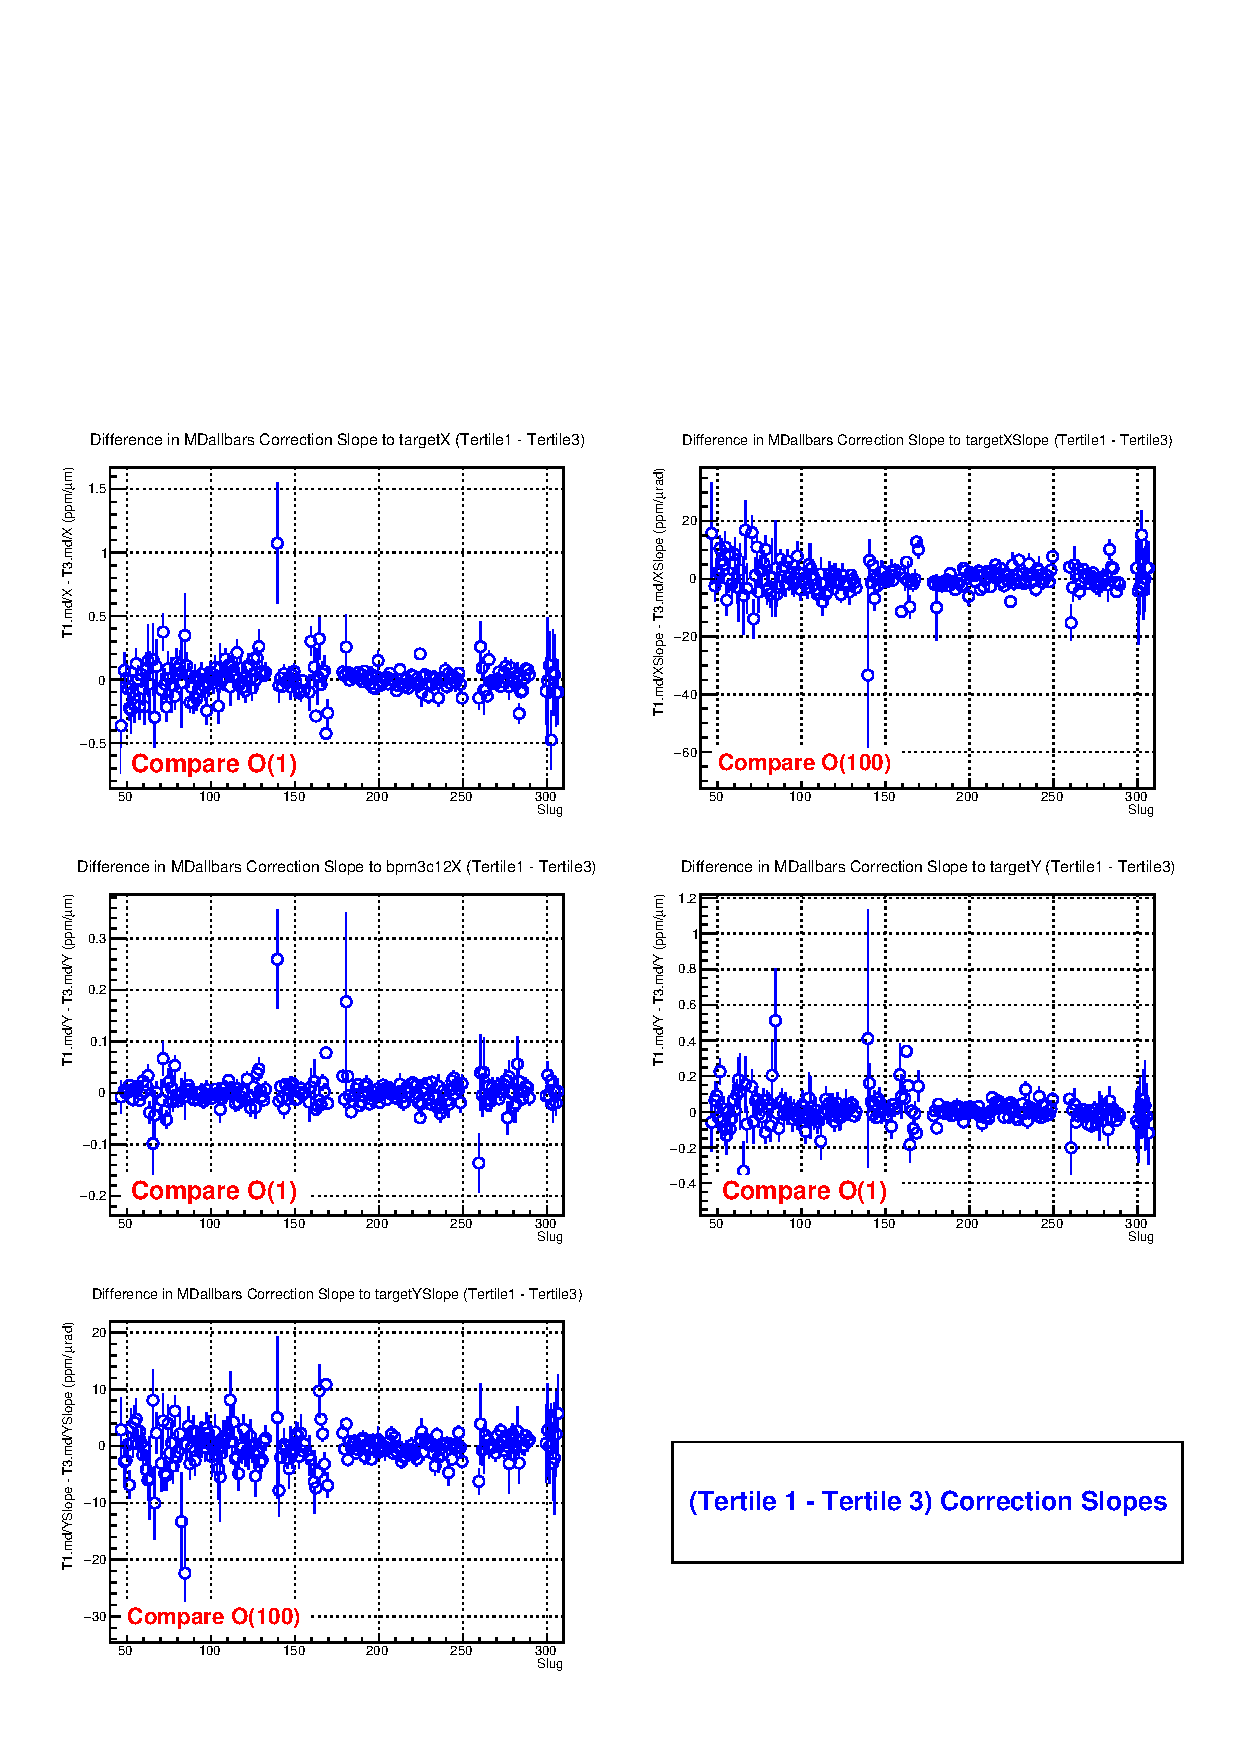
\includegraphics[width=5.6in]{Pictures/tertile1minus3Slope.pdf}}
\caption{Change in MDallbars correction slopes between tertiles 1 and 3. Each point represents the average for a given slug of data and the error bar is $\sigma/\sqrt{N}$. The ``pull plot'' distributions shown in Figure \ref{fig:tert_mdall_pull_plots} show that these differences are consistent with what is expected from statistics.}
\label{fig:tert_mdall_slope change}
\end{figure}

\begin{figure}[ht]

\centering
\framebox{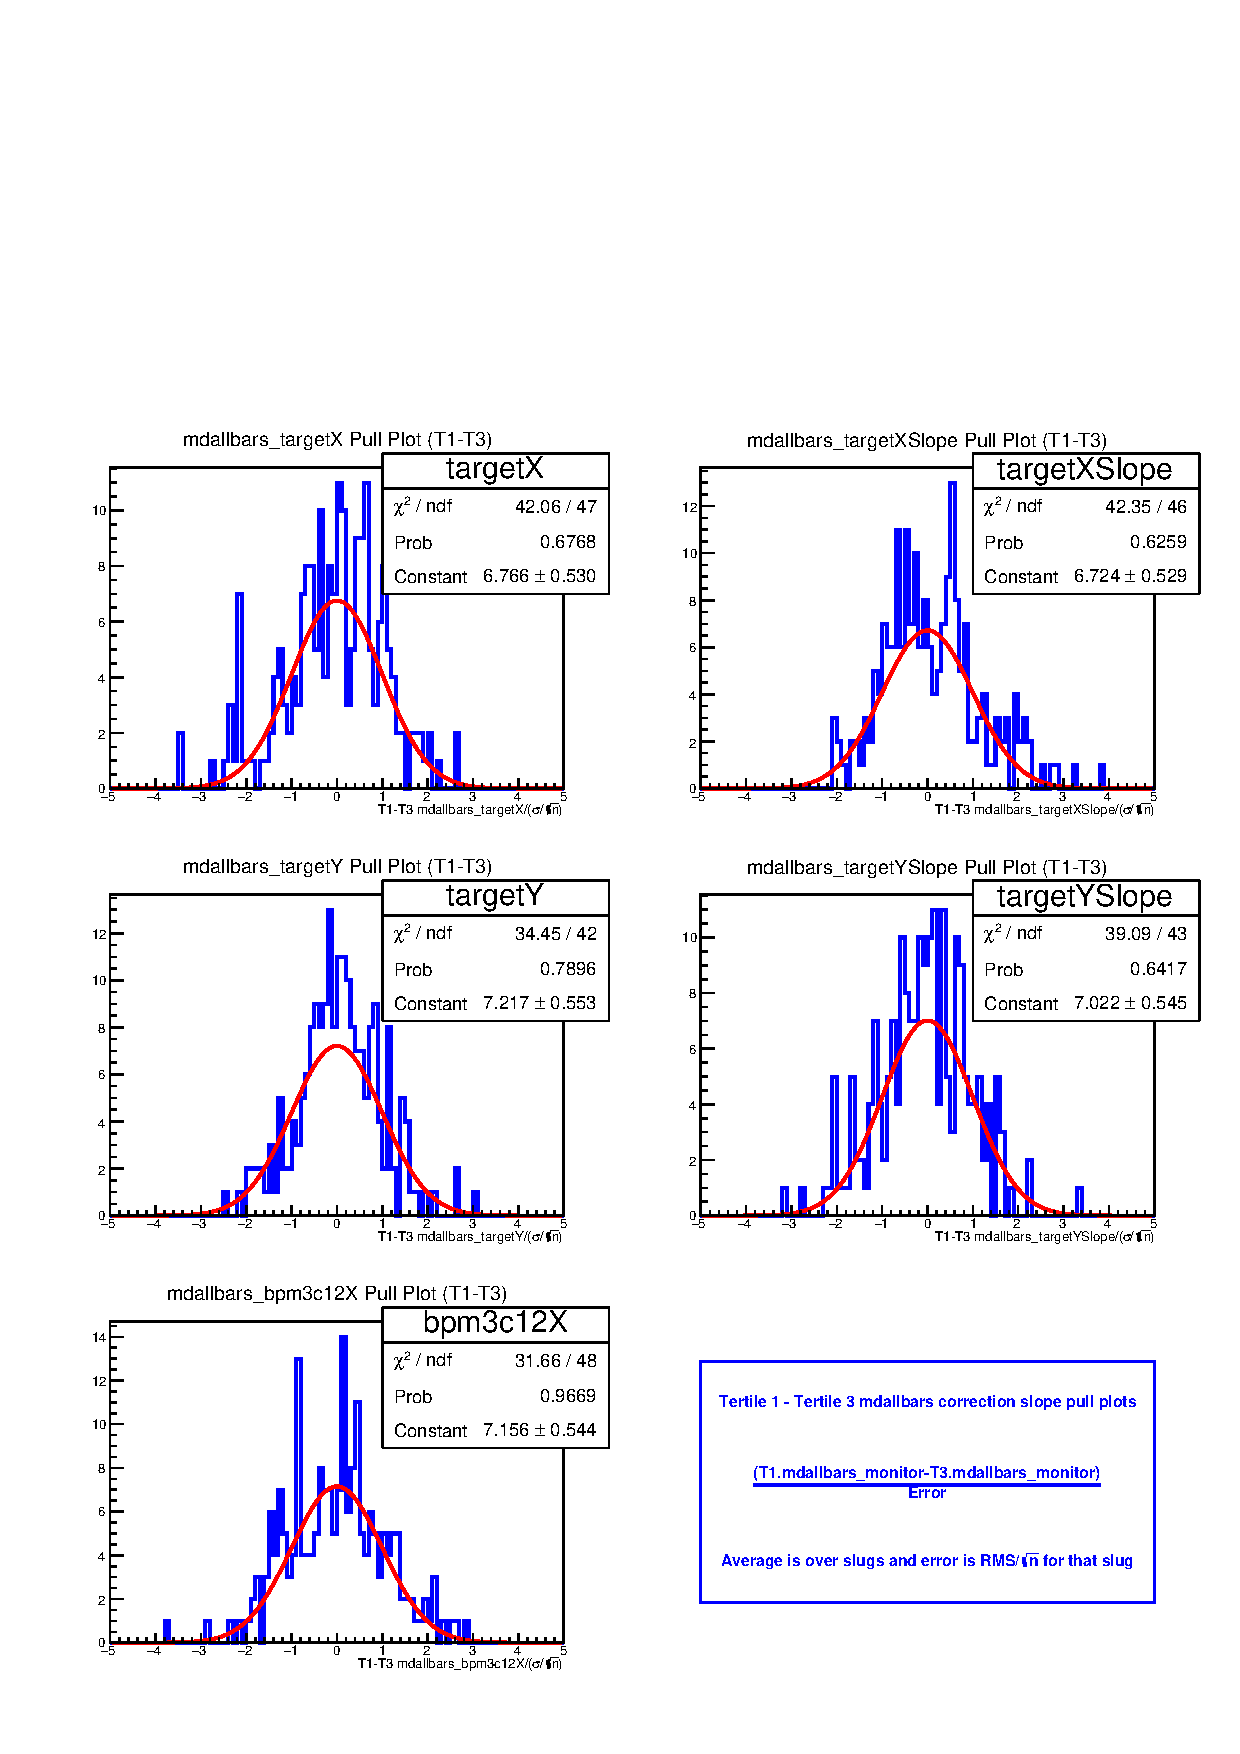
\includegraphics[width=5.6in]{Pictures/tertile_mdall_slopes_pull_plots.pdf}}
\caption{Pull distribution plots for difference in MDallbars to monitor correction slopes between tertiles 1 and 3. The histograms are the slug averages divided by their standard error. Pure statistical distributions (shown in red) are expected to have zero mean and unit standard deviation. The p-value of the fit of the distributions to the data indicate that the data are consistent with purely statistical deviations.}
\label{fig:tert_mdall_pull_plots}
\end{figure}

Figures \ref{fig:tert_coeffX} to  \ref{fig:tert_coeff3c12X} show the differences in the fit coefficients (sine and cosine fit amplitudes) between various tertiles, scaled by the total amplitude of the response for scale. ``Sine'' refers to the responses that are in phase with the modulation driving signal and ``Cosine'' to the responses that are $\pi/2$ out of phase with the driving signal.  The figure show a percent change in monitor and detector responses between tertiles. For example, the percent change in the in-phase response of ``targetX'' between tertiles 1 and 3 is given as
\begin{equation}
\frac{\Delta X_{sin}}{|X|}(\%)=100\%\times\frac{(X_{sin}^{(T1)}-X_{sin}^{(T3)})}{\sqrt{ \left(\frac{X_{sin}^{(T1)}+X_{sin}^{(T3)}}{2}\right)^2+\left(\frac{X_{cos}^{(T1)}+X_{cos}^{(T3)}}{2}\right)^2}},
\label{eq:fractional_tertile_change}
\end{equation}
where, for example $X_{sin}^{(T1)}$ is the sine response amplitude of targetX to a given type of modulation.

The results shown in figures \ref{fig:tert_coeffX} to  \ref{fig:tert_coeff3c12X}
suggest that for the most part, the FFB response as seen by the monitors is fairly stable over the modulation cycle time. When examining these plots it is helpful to remember that monitors less sensitive to a given modulation type may see larger percent changes but much smaller absolute changes. For example, we would expect targetX, targetXSlope and bpm3c12X to be most sensitive to X1 modulation with targetY and targetYSlope only marginally sensitive. Looking at the plots we can see percent level changes in  targetX, targetXSlope and bpm3c12X during X1 modulation. While targetY and targetYSlope see changes at the 10's of percent level during X1 modulation, the means of the distributions appear to be consistent with 0. Although one can point to seemingly large outliers where shifts of order 100\% occur, these outliers never occur in a monitor expected to have a large response to a given modulation type. These observations lead to the following conclusions:
\begin{itemize}
\item{The monitors that are expected to be sensitive to a given type of modulation appear to have a relatively stable response at the few percent level when different ``slices'' of the modulation cycles are compared.}
\item{Monitors not expected to be sensitive to a given type of modulation do not show large (greater than a few percent) systematic shifts in response when different ``slices'' of the modulation cycles are compared.}
\item{The largest shifts occur during energy modulation when the FFB system is paused. Shifts during this time must be attributed to instability in the energy response, not to FFB. It is conceivable that some unknown feedback system such as MOMOD remains active during energy modulation and creates the energy instability.} 
\end{itemize}

Figures \ref{fig:tert_md_coeff_coil0} to \ref{fig:tert_md_coeff_coil9} show similar small variations between tertile 1 and tertile 3 in the main detector responses. 

It may be observed, however, that the stability observed in the slopes appears to be greater than that in the monitor and detector coefficients. In fact, they appear to be consistent with statistics. How is the stability of the detector to monitor correction slopes to be understood in the light of the larger instability of the monitor and detector coefficients? Although stability is desired because any noise will increase the uncertainty, perfect stability is not critical to the modulation analysis procedure. In the end, the periodic modulation is only used to determine a relationship between the detectors and monitors and all that is necessary is that there be a well-determined average response of both monitors and detectors over the cycles. It is useful to remember that this whole analysis assumes that the detectors and monitors are linear and only removes the linear response. Beyond that there is no condition on the stability of the driving system built into Equations \ref{eq:det_to_coil} or \ref{eq:chisquaresolution_no_variance}. The basic conditions for success of the modulation analysis method are:
\begin{itemize}
\item{Modulation must span space of beam distortion modes: \\The 5 main ``distortion'' modes are thought to be horizontal and vertical motion, horizontal and vertical angle and energy. The beam must be driven in such a way that all 5 parameters are modulated.}
\item{Monitor set must also span this beam distortion space:\\ The combined set of monitors must have a collective sensitivity to the full phase space in which the beam is driven by the modulation coils. We must have monitors that are sensitive to the five main beam parameters.}
\item{A calibration signal precisely proportional to and in phase with the coil driving signal must be available: \\
Unlike linear regression, monitor and detector responses are not directly compared. Instead the response of each is found relative to the calibration signal. For the Qweak modulation system, a sinusoidal signal sent to the coils (both air coil magnets and the RF cavity) was used to drive beam motion. The physical calibration signal came in the form of a sawtooth wave synchronous with the drive signal to the coils. The sawtooth wave was then translated into a modulation phase and our actual calibration signal was the sine and cosine of this phase. Without this information about the drive signal, the only possible correction for trajectory related false asymmetries would be linear regression.}
\item{The response to the motion must be well-determined in both the monitors and detectors. This is not the same as saying it must non-zero.}
\end{itemize}

An unstable response amplitude will create greater uncertainty in the determination of correction slopes, but it will not in general bias the results unless there exists some instability that is somehow coherent with the driving signal. Since the detectors and the monitors used to correct them both respond to the same unstable behavior, the slopes should be the same within error for both a stable response and a slowly changing response amplitude and this is consistent with our observations.


\begin{landscape}
\begin{figure}[t]

\centering
\framebox{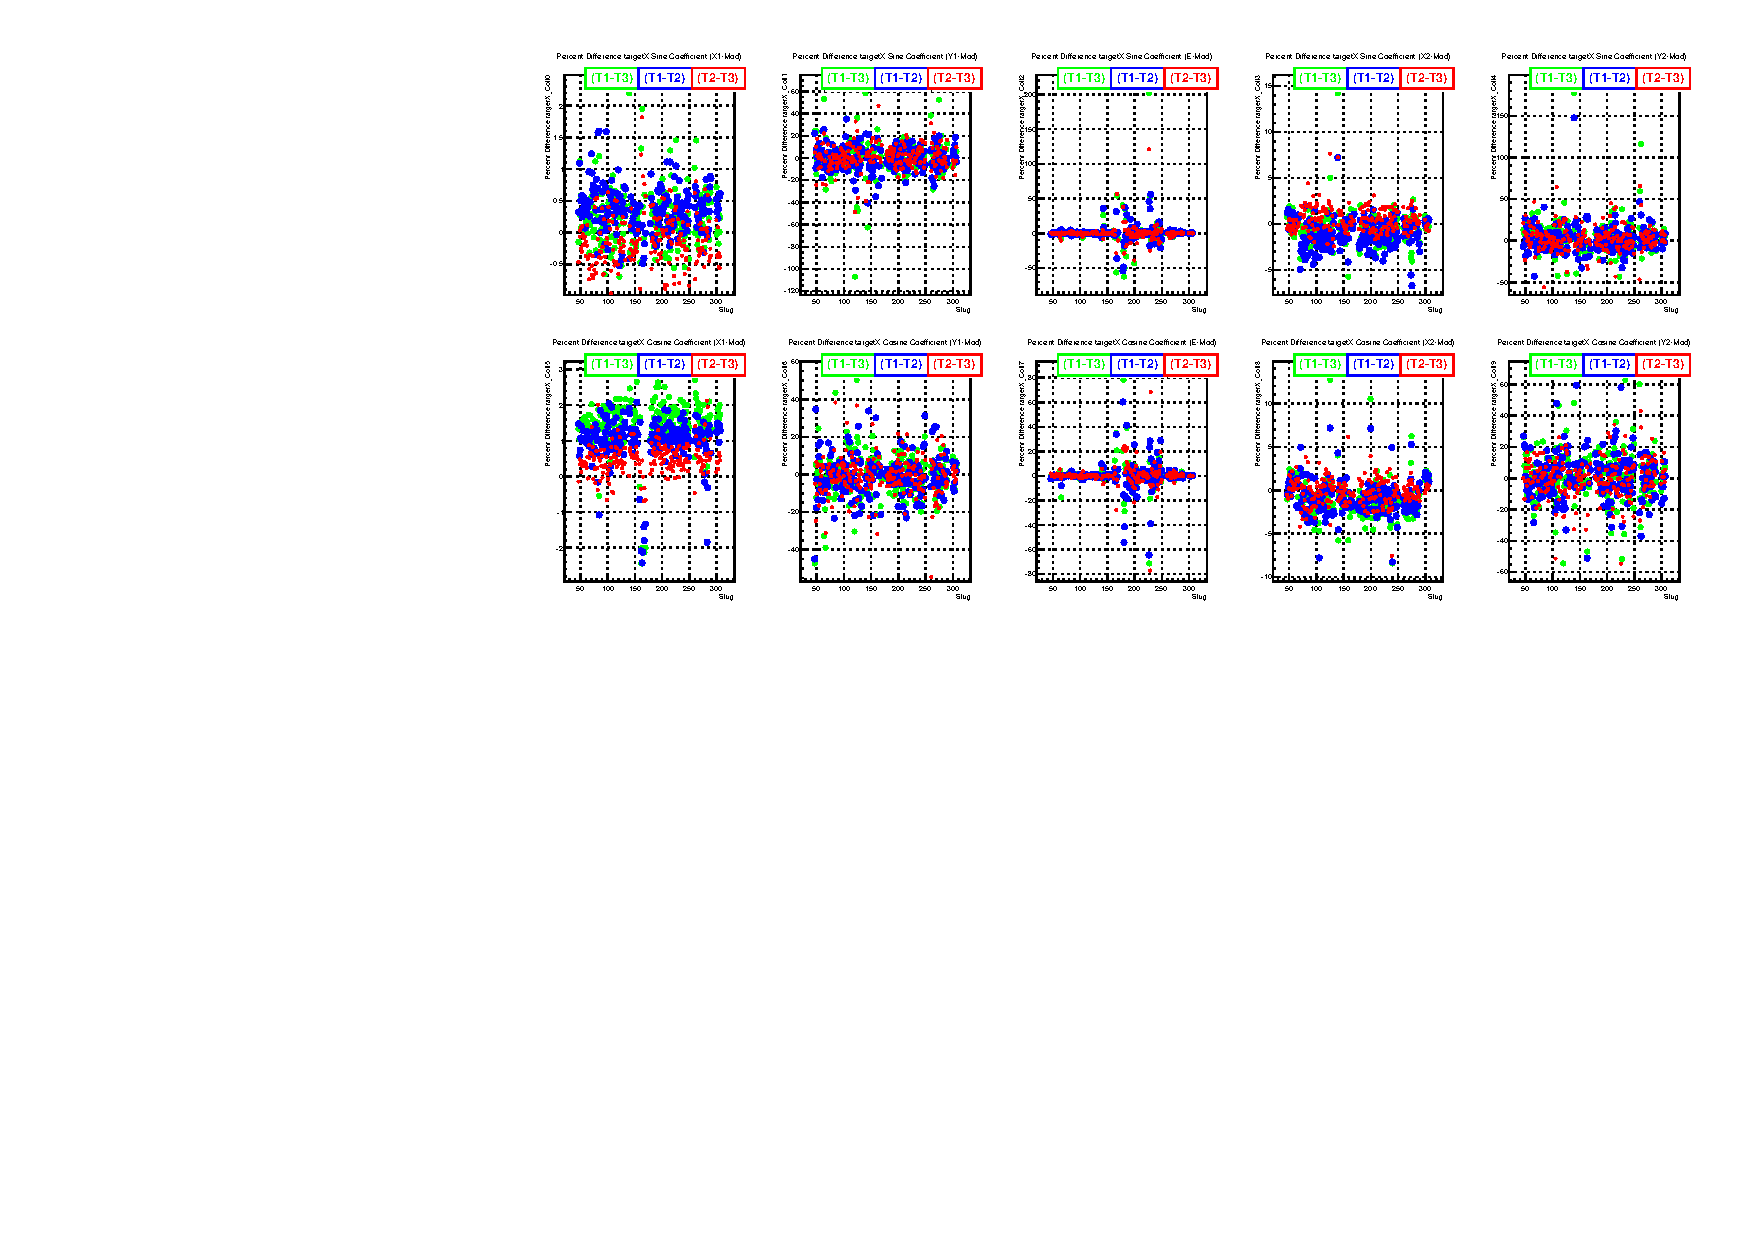
\includegraphics[width=8.9in]{Pictures/tertile_percent_coefficient_change_targetX.pdf}}
\caption{Percent change in targetX response between data tertiles. See Equation \ref{eq:fractional_tertile_change} for an explanation of the percent change shown.}

\label{fig:tert_coeffX}
\end{figure}

\begin{figure}[t]

\centering
\framebox{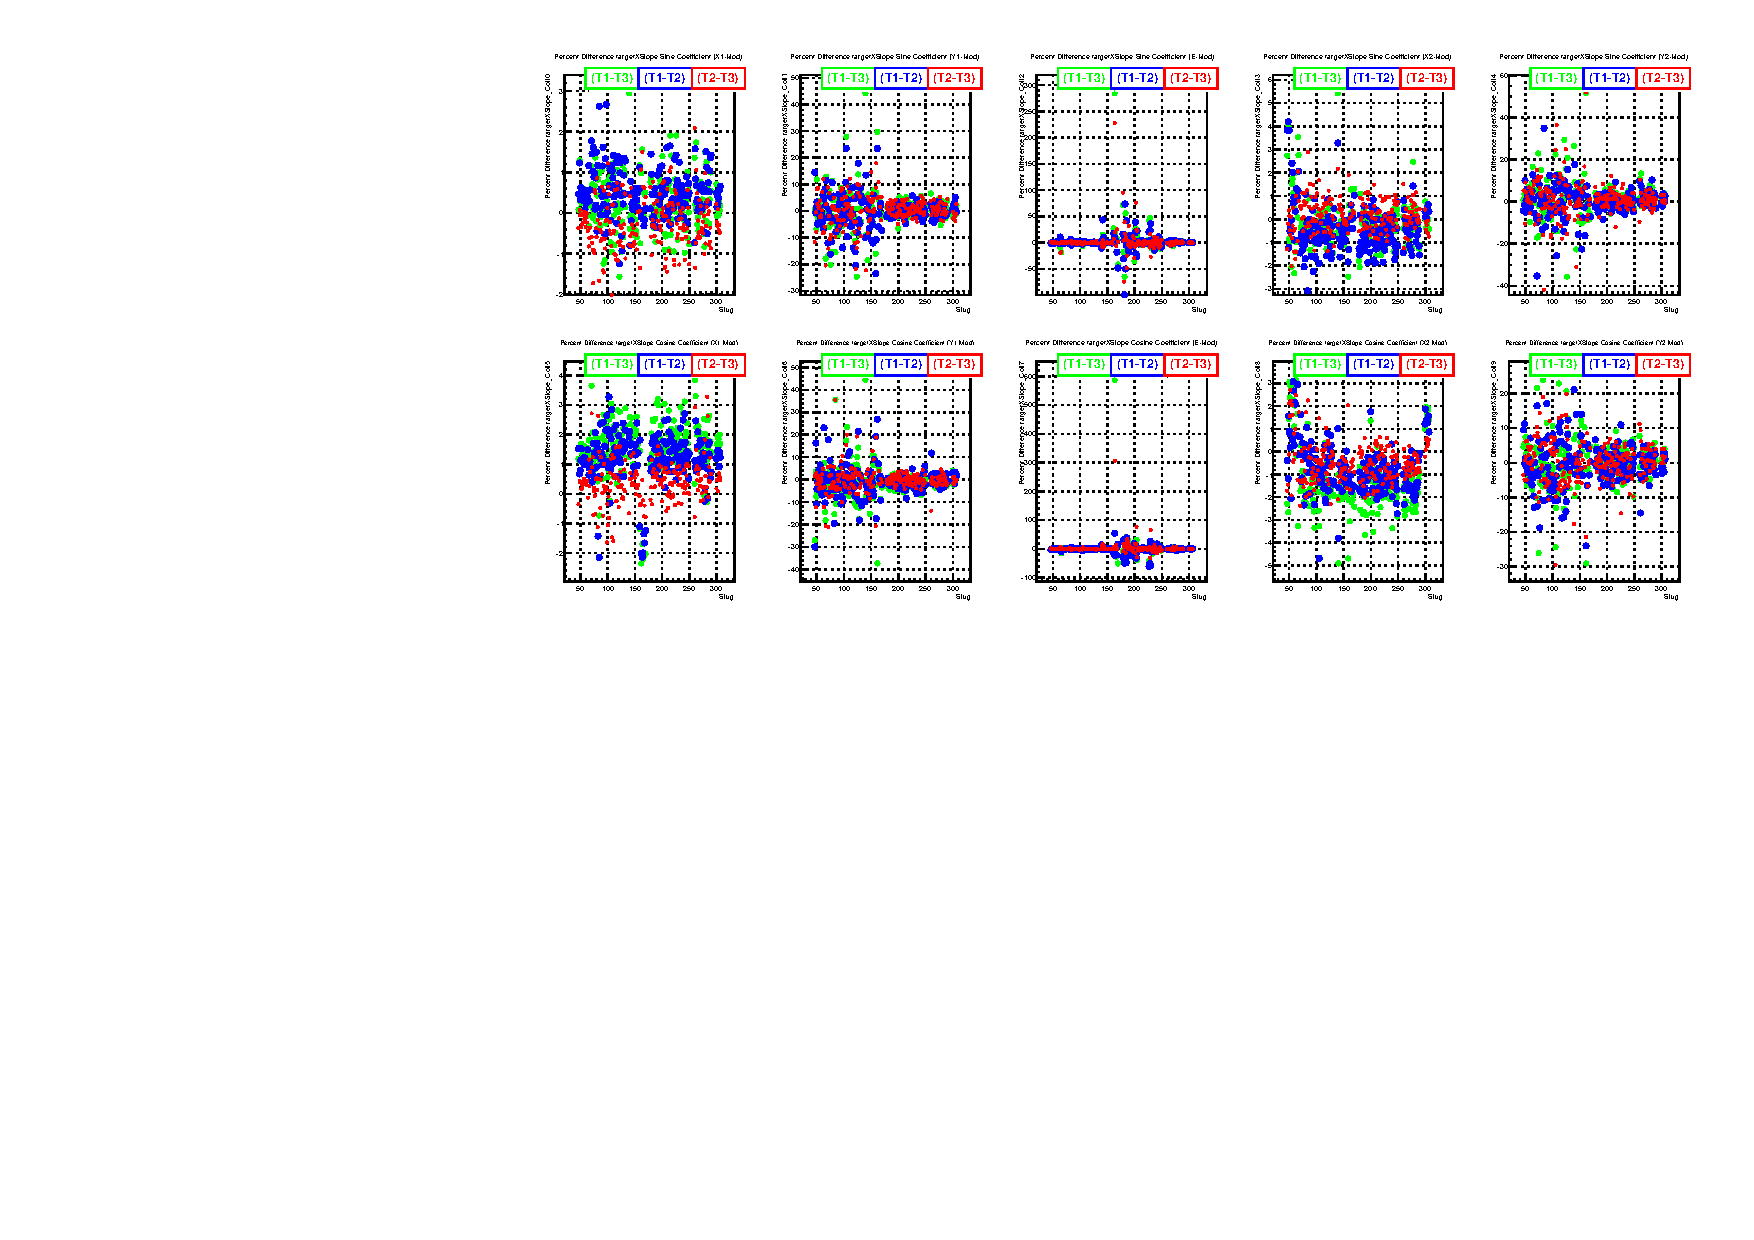
\includegraphics[width=8.9in]{Pictures/tertile_percent_coefficient_change_targetXSlope.pdf}}
\caption{Percent change in targetXSlope response between data tertiles. See Equation \ref{eq:fractional_tertile_change} for an explanation of the percent change shown.}

\label{fig:tert_coeffXSlope}
\end{figure}
\begin{figure}[t]

\centering
\framebox{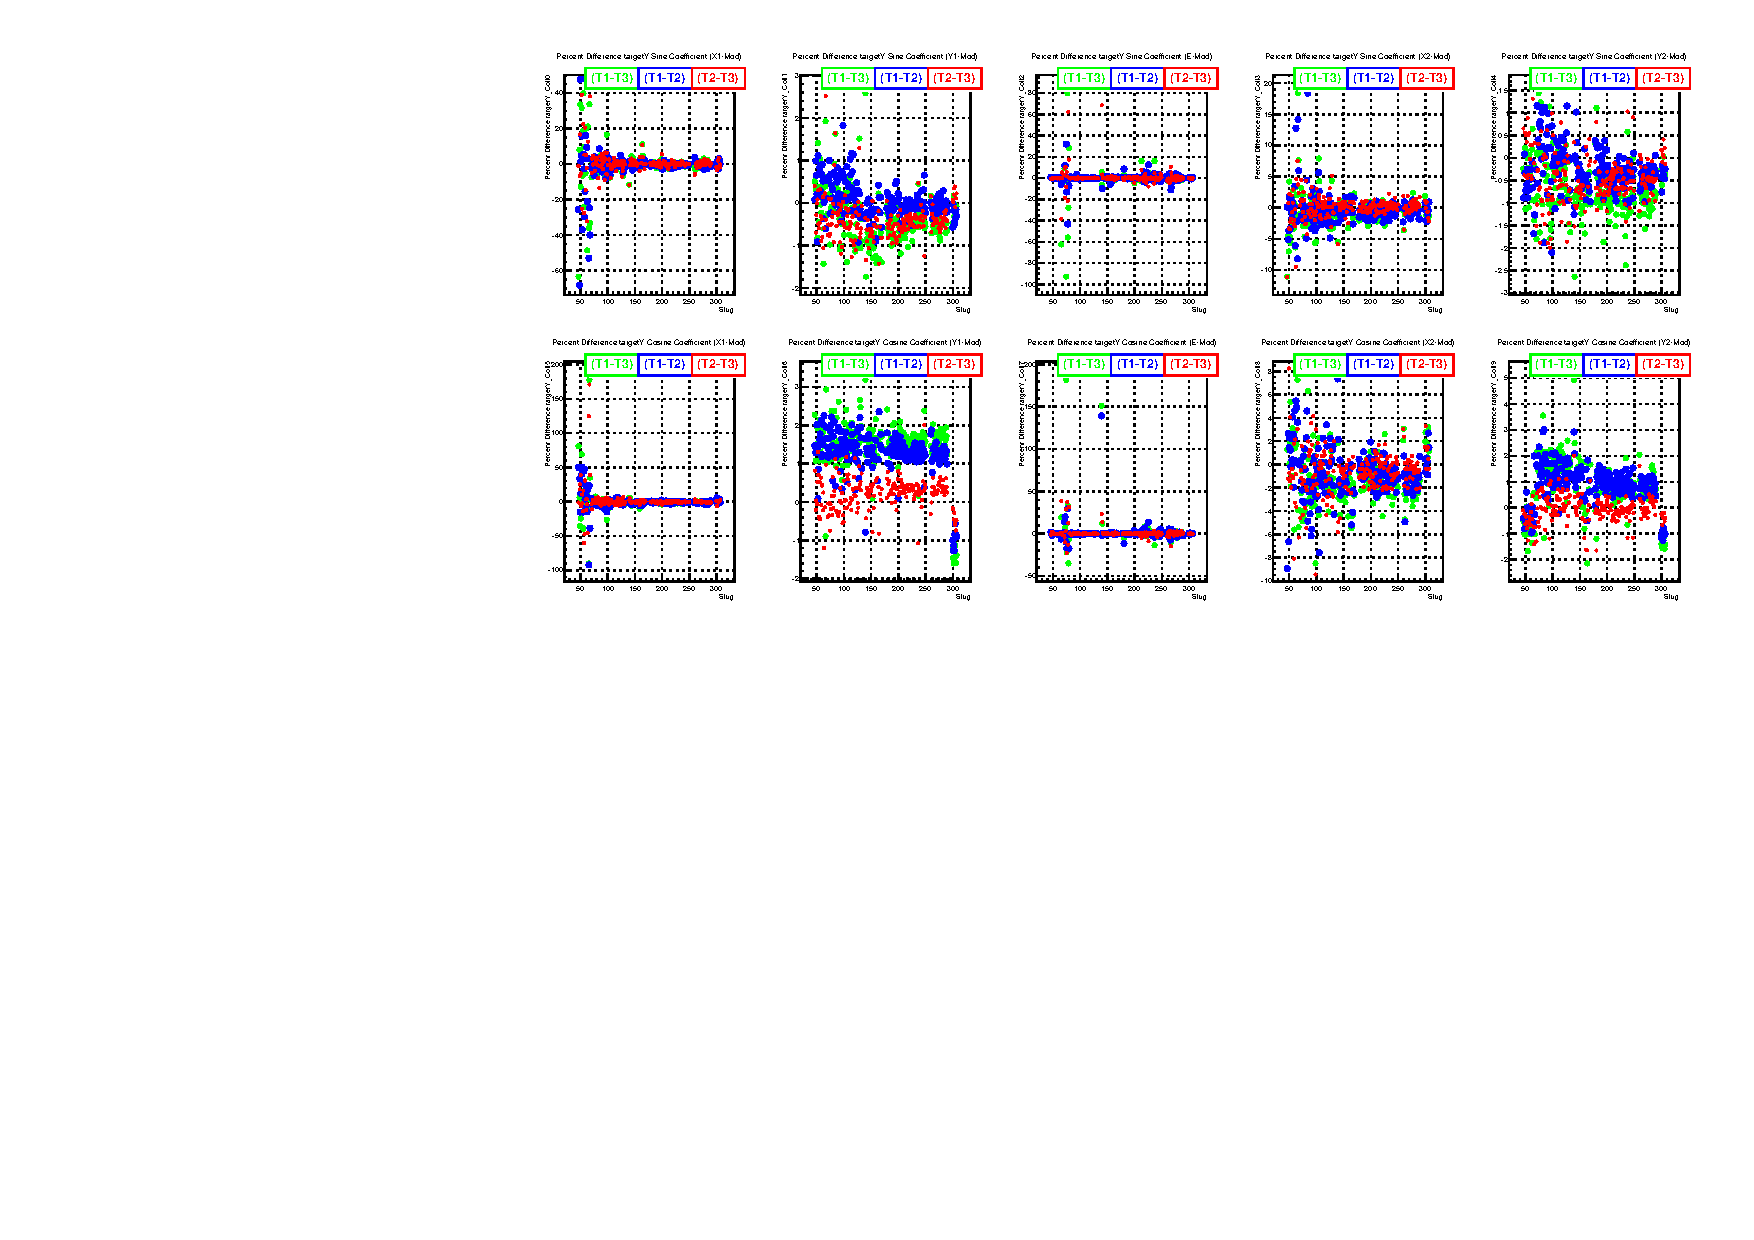
\includegraphics[width=8.9in]{Pictures/tertile_percent_coefficient_change_targetY.pdf}}
\caption{Percent change in targetY response between data tertiles. See Equation \ref{eq:fractional_tertile_change} for an explanation of the percent change shown.}

\label{fig:tert_coeffY}
\end{figure}

\begin{figure}[t]

\centering
\framebox{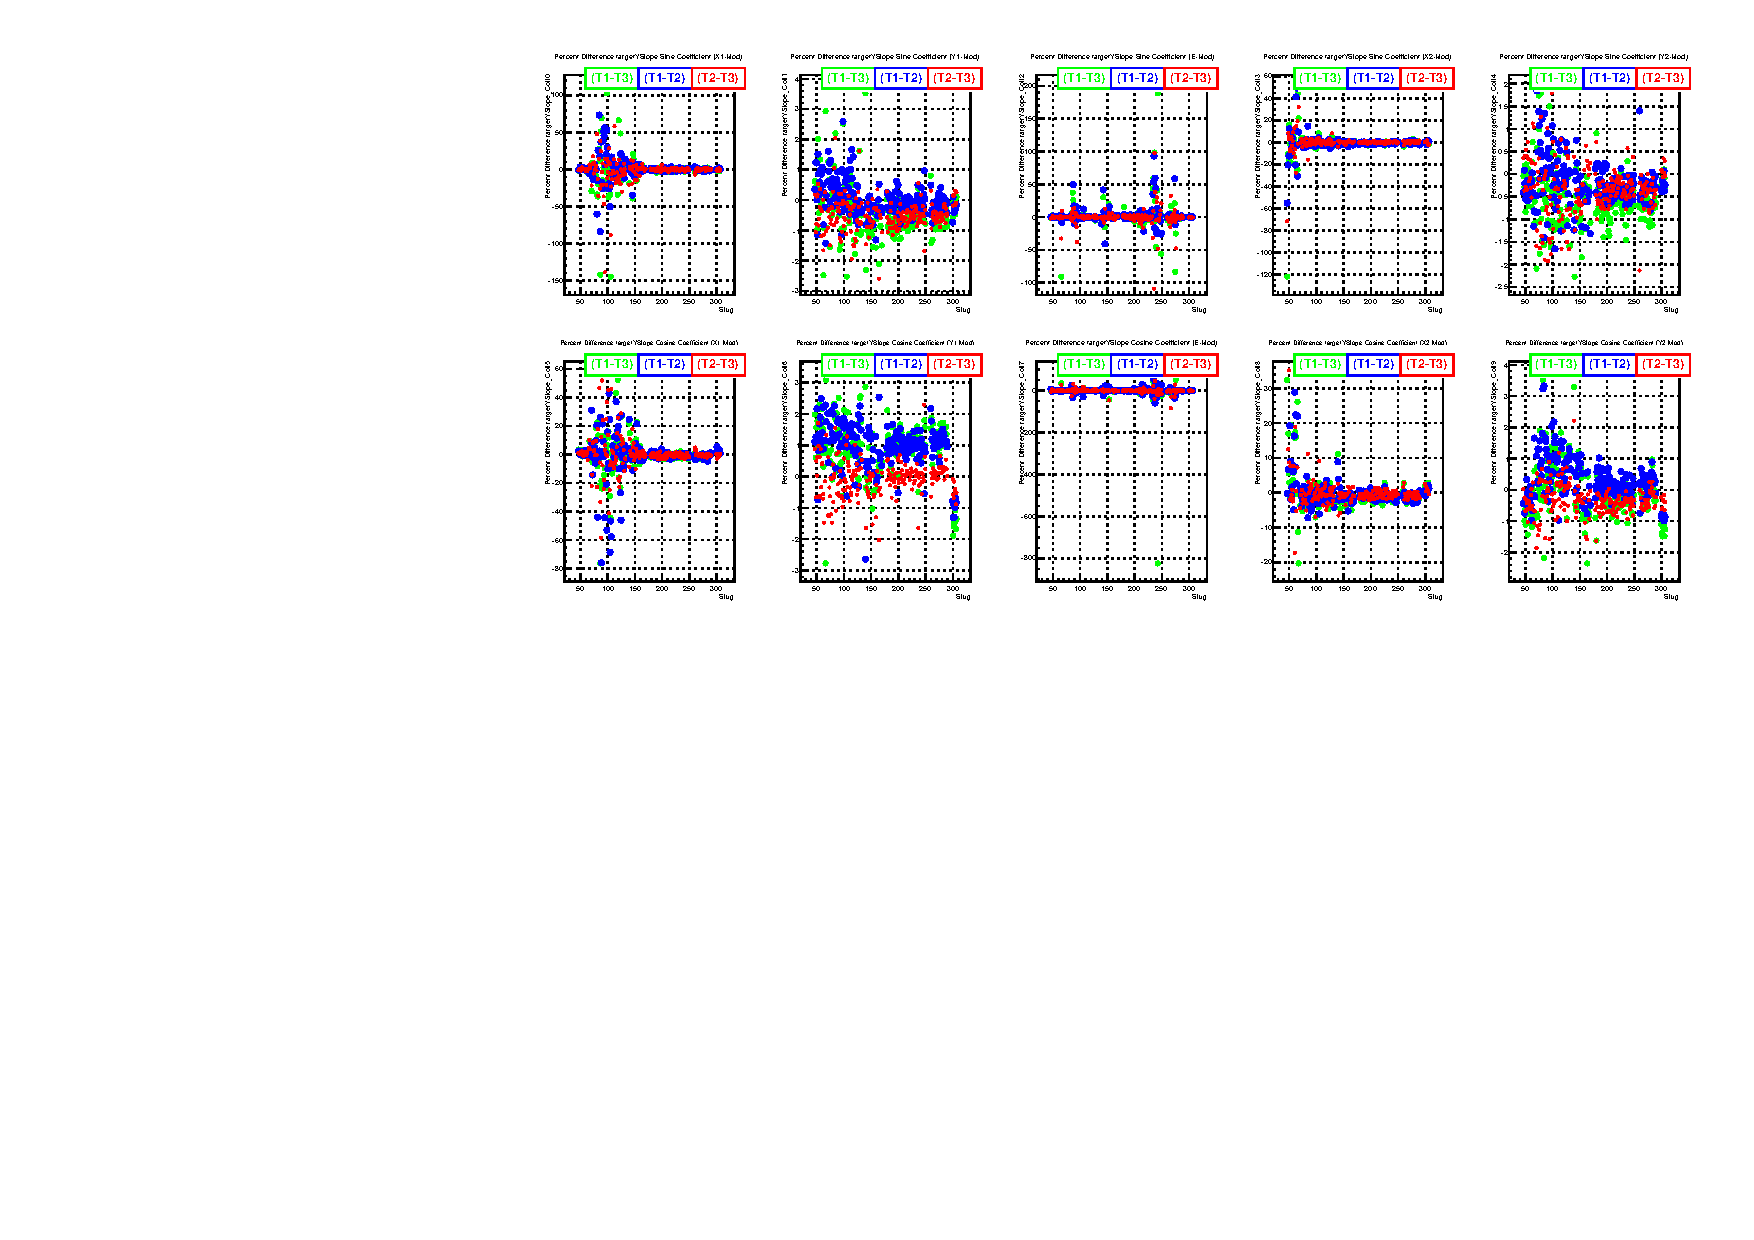
\includegraphics[width=8.9in]{Pictures/tertile_percent_coefficient_change_targetYSlope.pdf}}
\caption{Percent change in targetYSlope response between data tertiles. See Equation \ref{eq:fractional_tertile_change} for an explanation of the percent change shown.}

\label{fig:tert_coeffYSlope}
\end{figure}
\begin{figure}[t]

\centering
\framebox{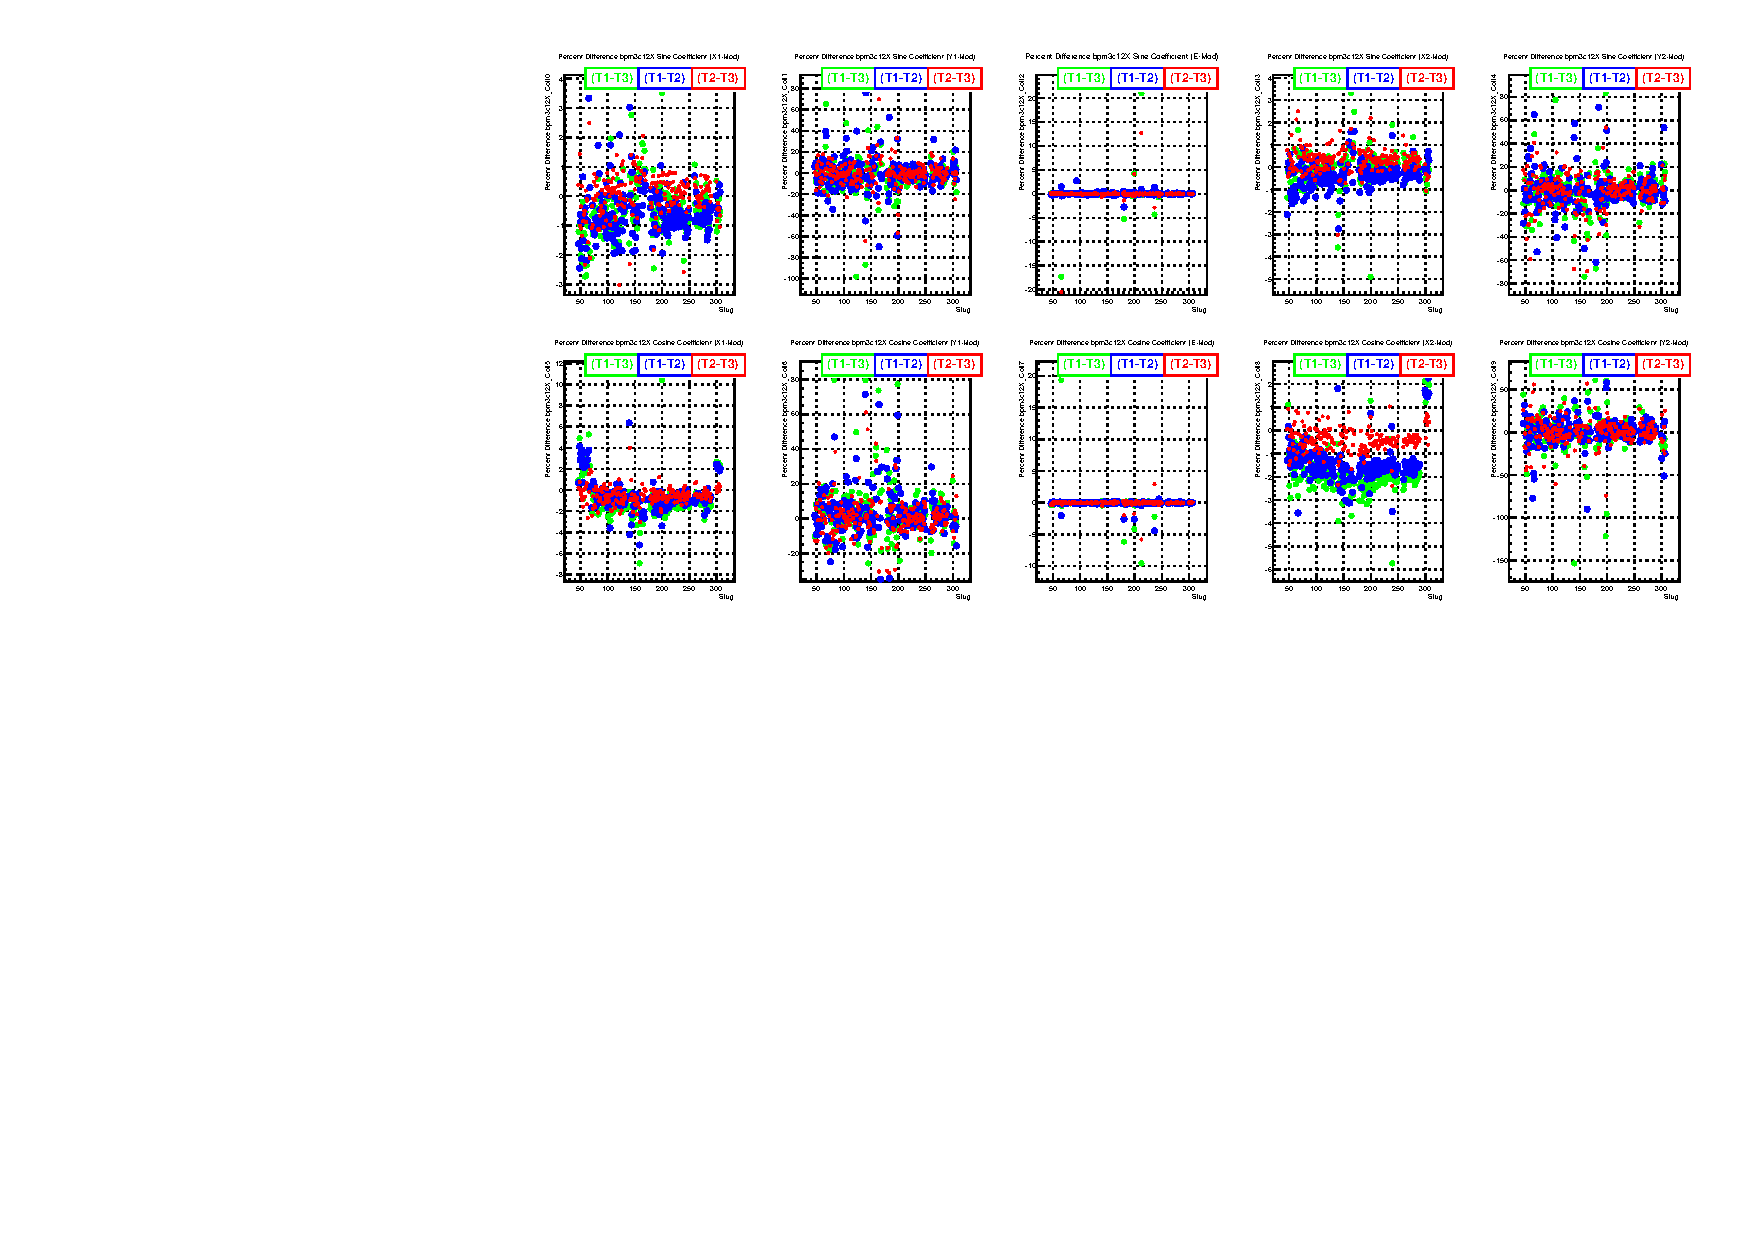
\includegraphics[width=8.9in]{Pictures/tertile_percent_coefficient_change_bpm3c12X.pdf}}
\caption{Percent change in bpm3c12X response between data tertiles. See Equation \ref{eq:fractional_tertile_change} for an explanation of the percent change shown.}

\label{fig:tert_coeff3c12X}
\end{figure}
\end{landscape}

\begin{figure}[h]

\centering
\framebox{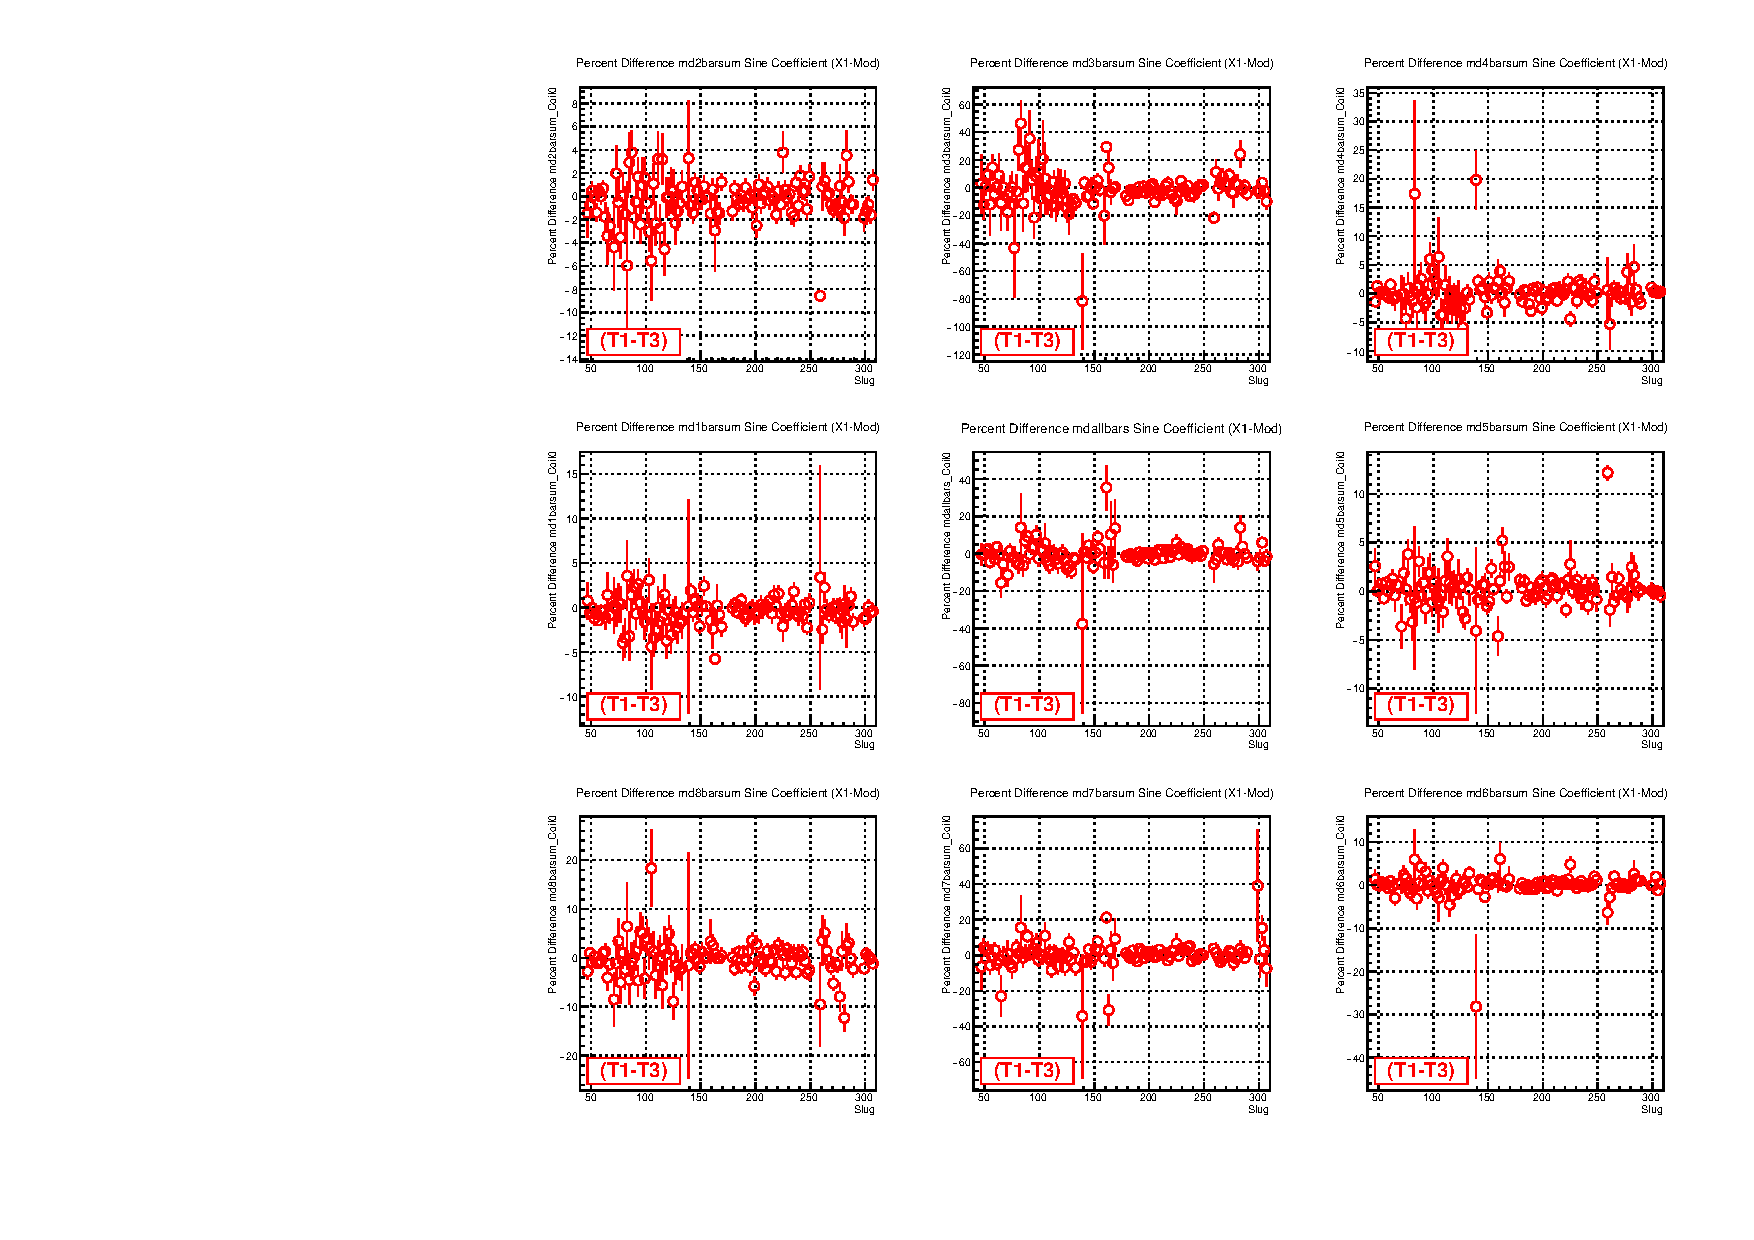
\includegraphics[width=5.6in]{Pictures/T1minusT3_mdallbars_coefficients_Coil0.pdf}}
\caption{Percent change in the in-phase (sine) main detector response between data tertiles 1 and 3 during X1-modulation (coil 0). See Equation \ref{eq:fractional_tertile_change} for an explanation of the percent change shown.}
\label{fig:tert_md_coeff_coil0}
\end{figure}
\begin{figure}[h]

\centering
\framebox{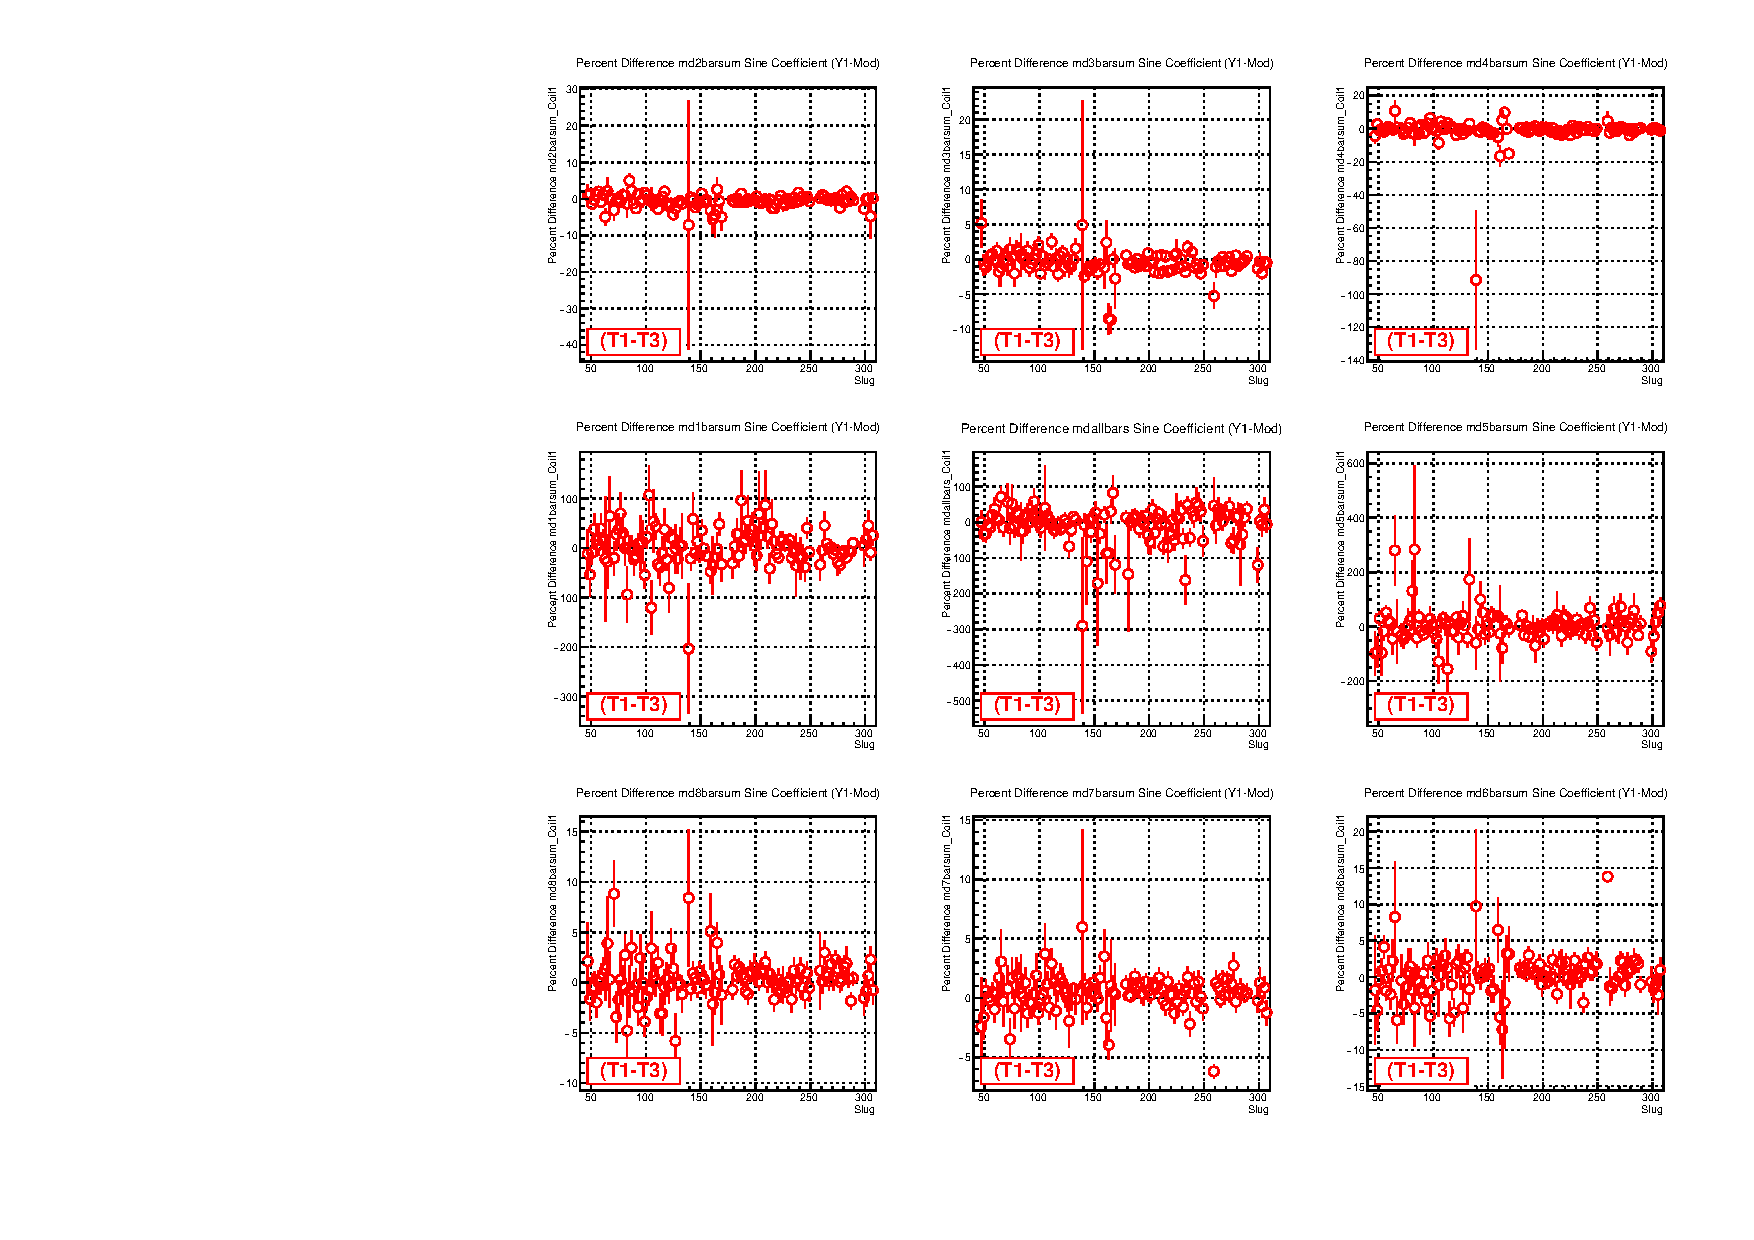
\includegraphics[width=5.6in]{Pictures/T1minusT3_mdallbars_coefficients_Coil1.pdf}}
\caption{Percent change in the in-phase (sine) main detector response between data tertiles 1 and 3 during Y1-modulation (coil 1). See Equation \ref{eq:fractional_tertile_change} for an explanation of the percent change shown.}
\label{fig:tert_md_coeff_coil1}
\end{figure}
\begin{figure}[h]

\centering
\framebox{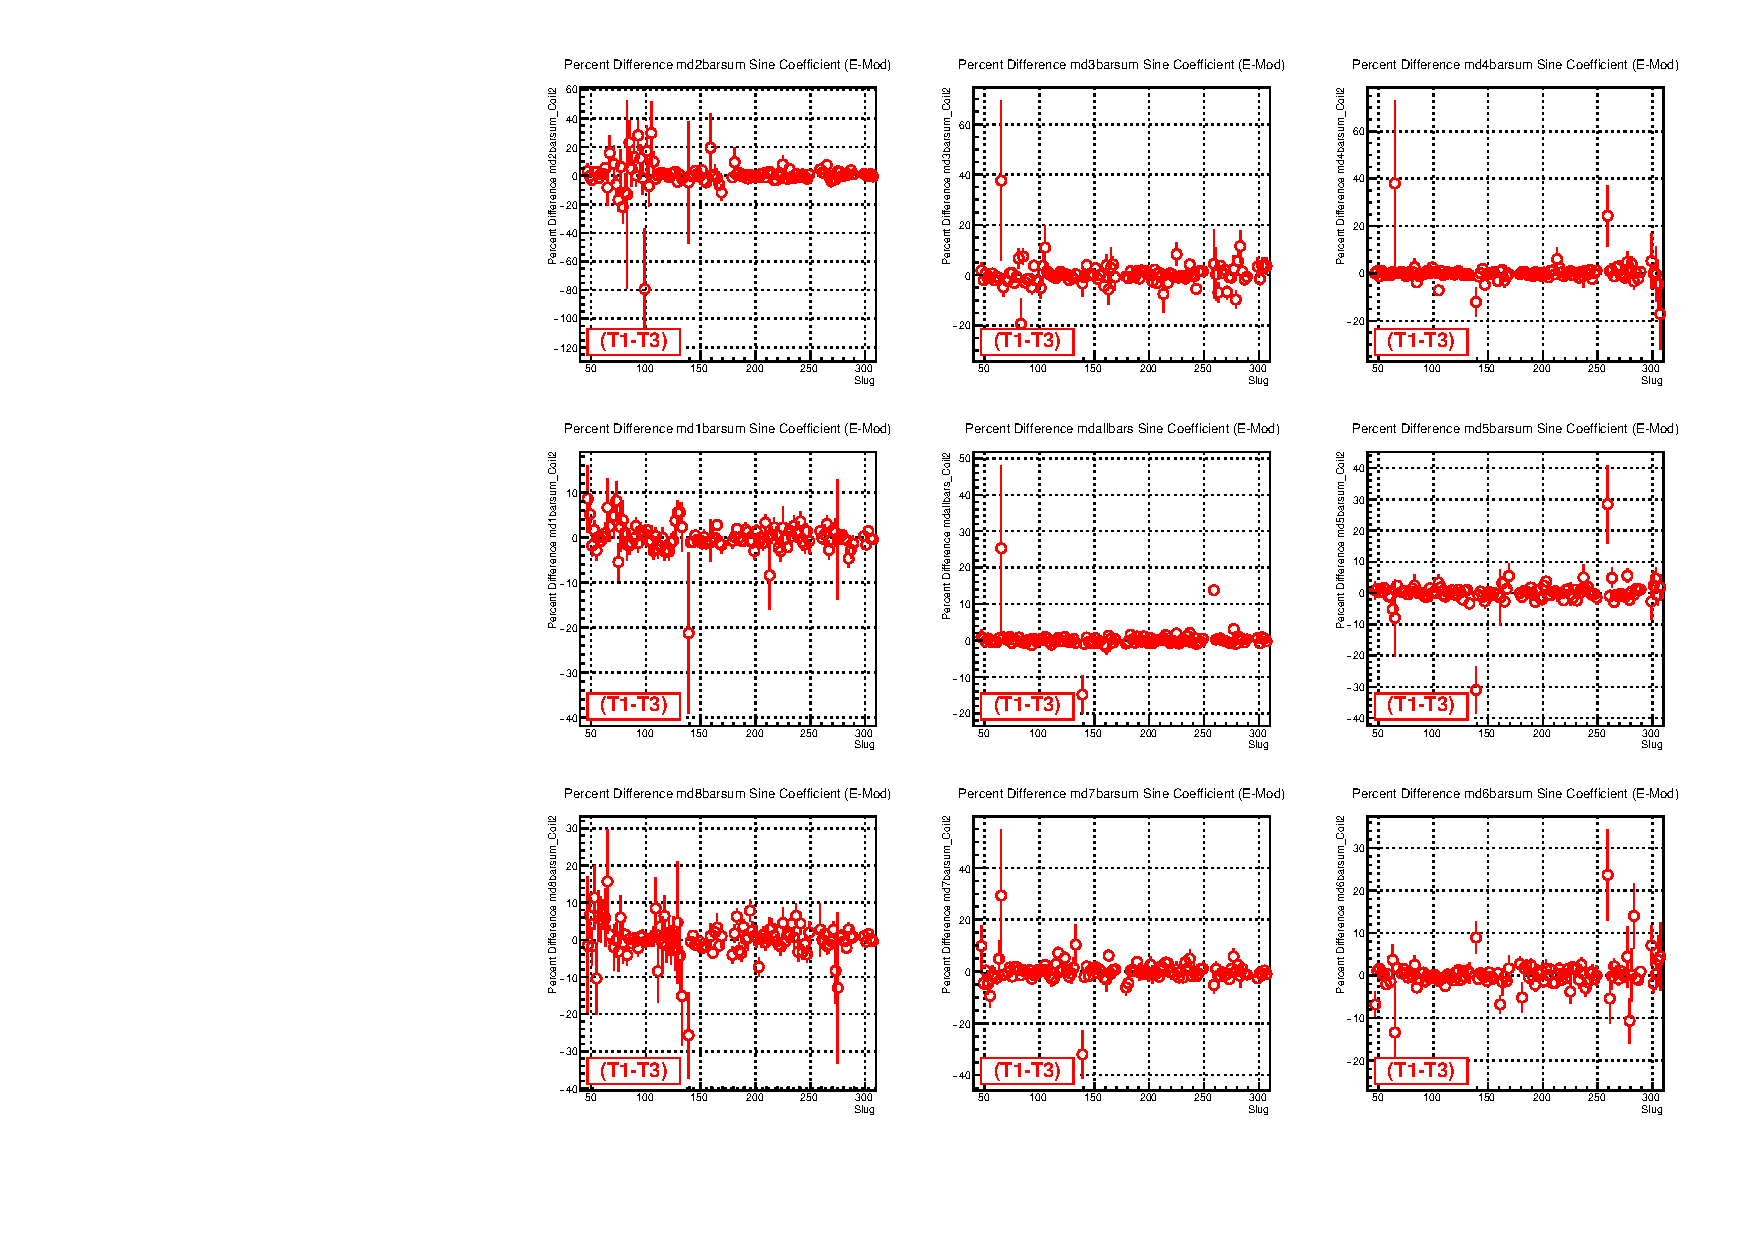
\includegraphics[width=5.6in]{Pictures/T1minusT3_mdallbars_coefficients_Coil2.pdf}}
\caption{Percent change in the in-phase (sine) main detector response between data tertiles 1 and 3 during energy modulation(coil 2) . See Equation \ref{eq:fractional_tertile_change} for an explanation of the percent change shown.}
\label{fig:tert_md_coeff_coil2}
\end{figure}
\begin{figure}[h]

\centering
\framebox{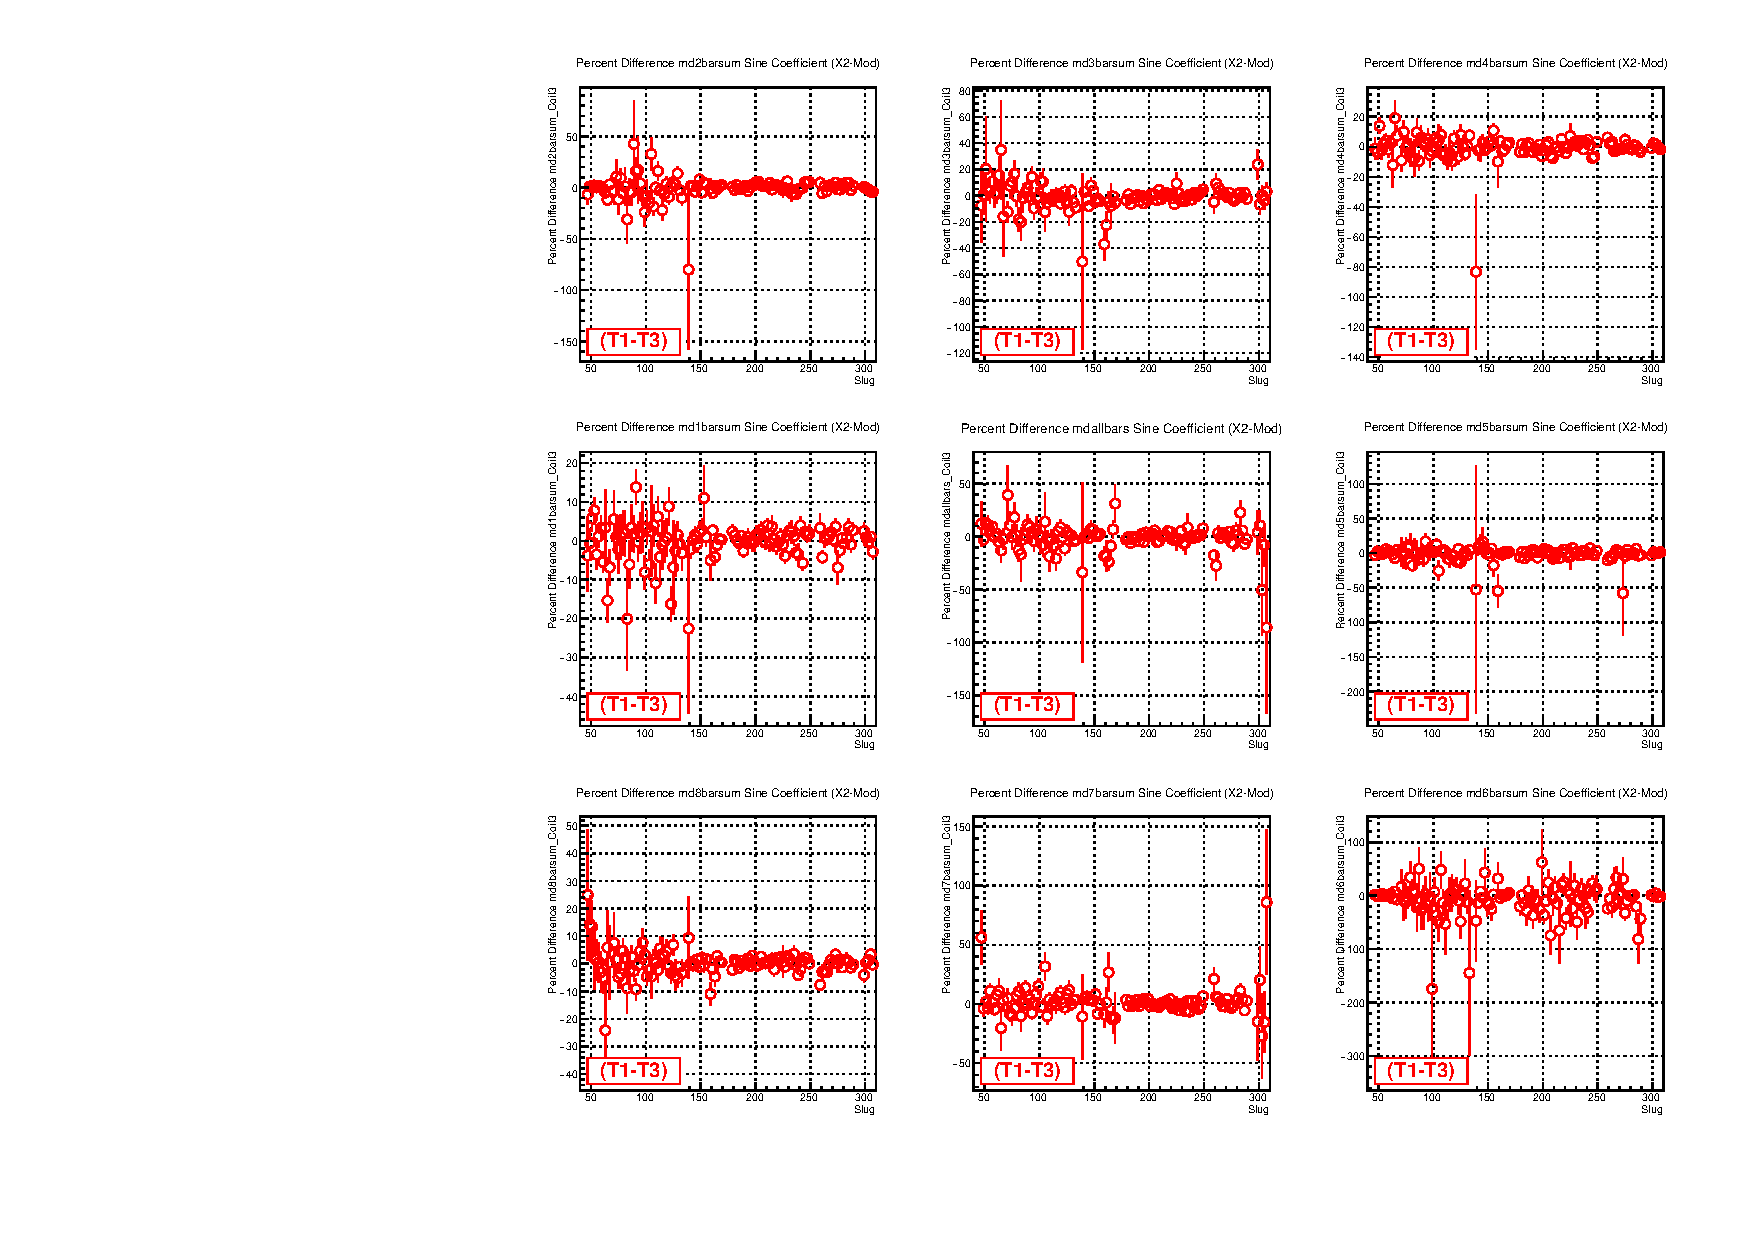
\includegraphics[width=5.6in]{Pictures/T1minusT3_mdallbars_coefficients_Coil3.pdf}}
\caption{Percent change in the in-phase (sine) main detector response between data tertiles 1 and 3 during X2-modulation (coil 3). See Equation \ref{eq:fractional_tertile_change} for an explanation of the percent change shown.}
\label{fig:tert_md_coeff_coil3}
\end{figure}
\begin{figure}[h]

\centering
\framebox{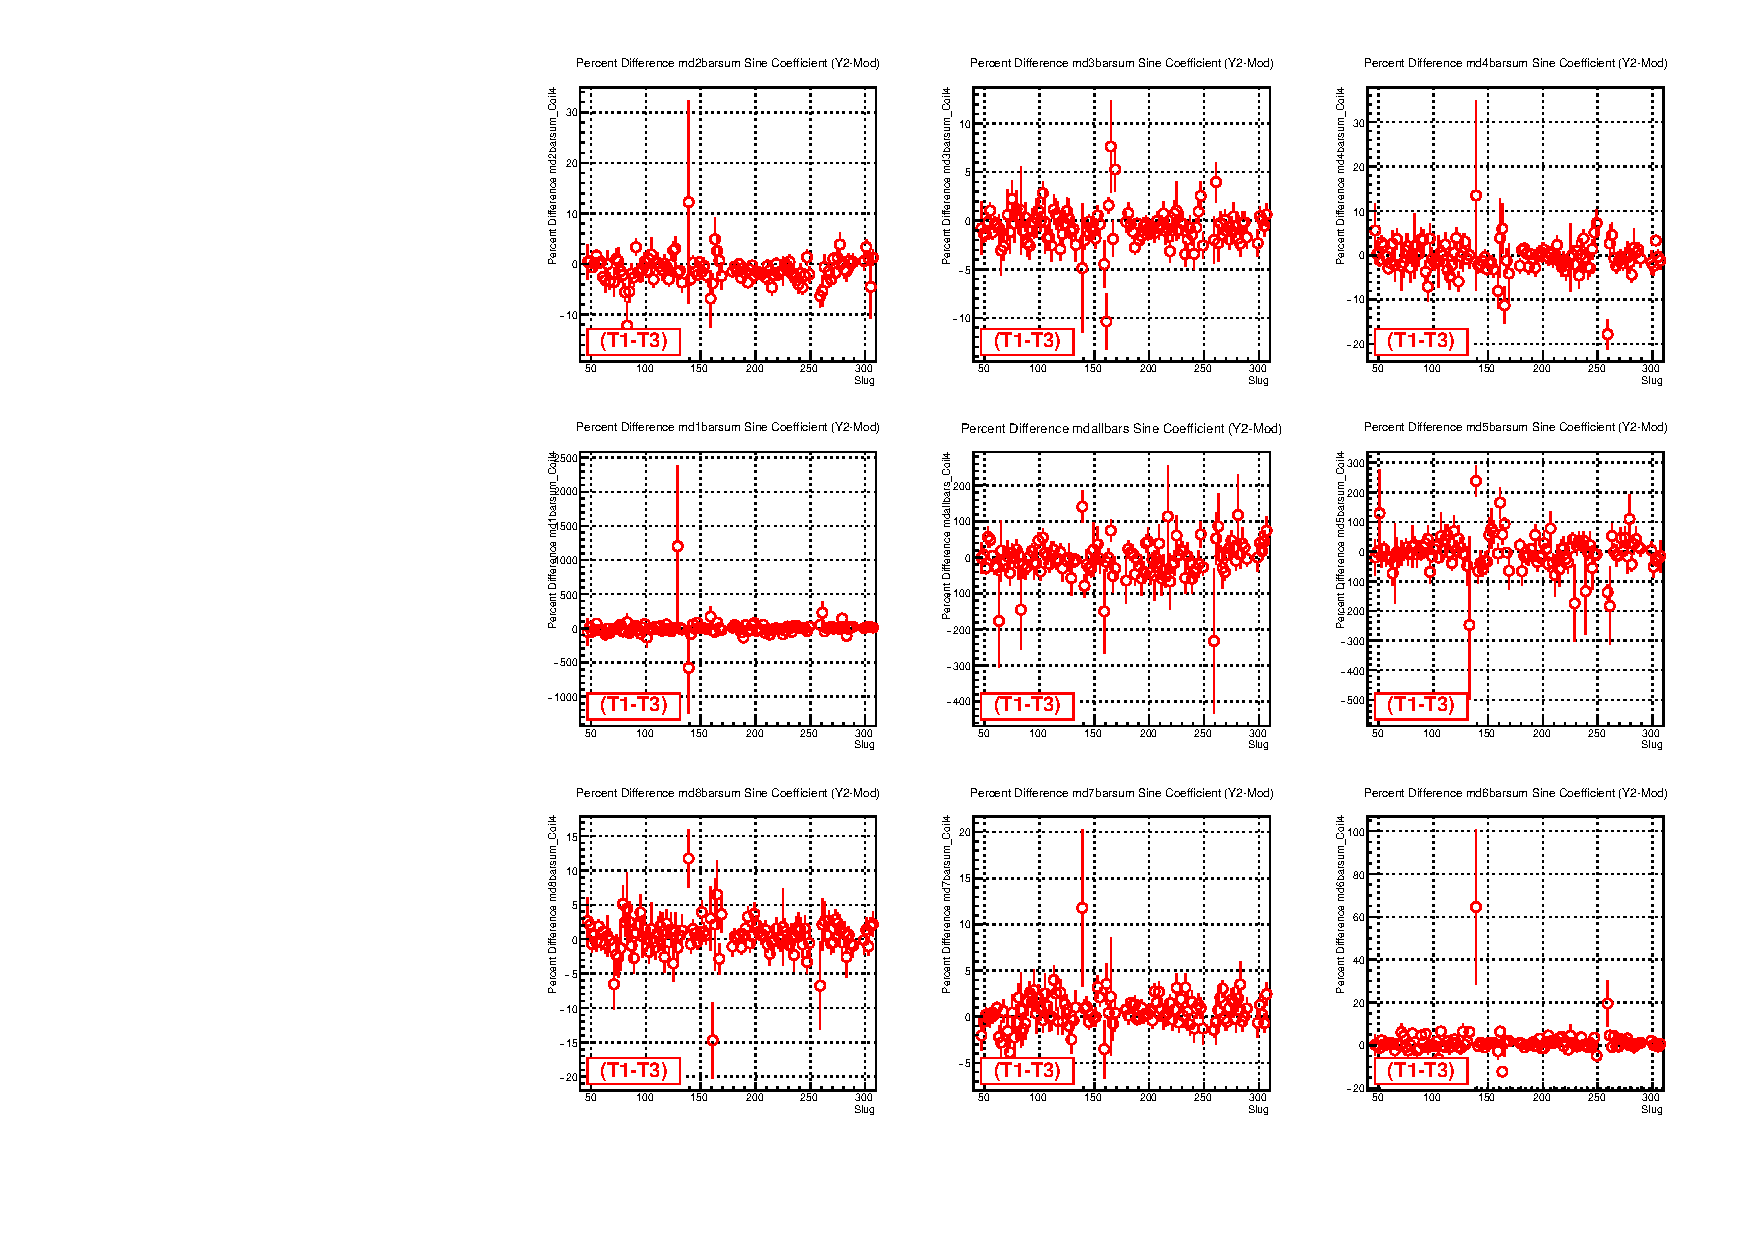
\includegraphics[width=5.6in]{Pictures/T1minusT3_mdallbars_coefficients_Coil4.pdf}}
\caption{Percent change in the in-phase (sine) main detector response between data tertiles 1 and 3 during Y2-modulation (coil 4). See Equation \ref{eq:fractional_tertile_change} for an explanation of the percent change shown.}
\label{fig:tert_md_coeff_coil4}
\end{figure}
\begin{figure}[h]

\centering
\framebox{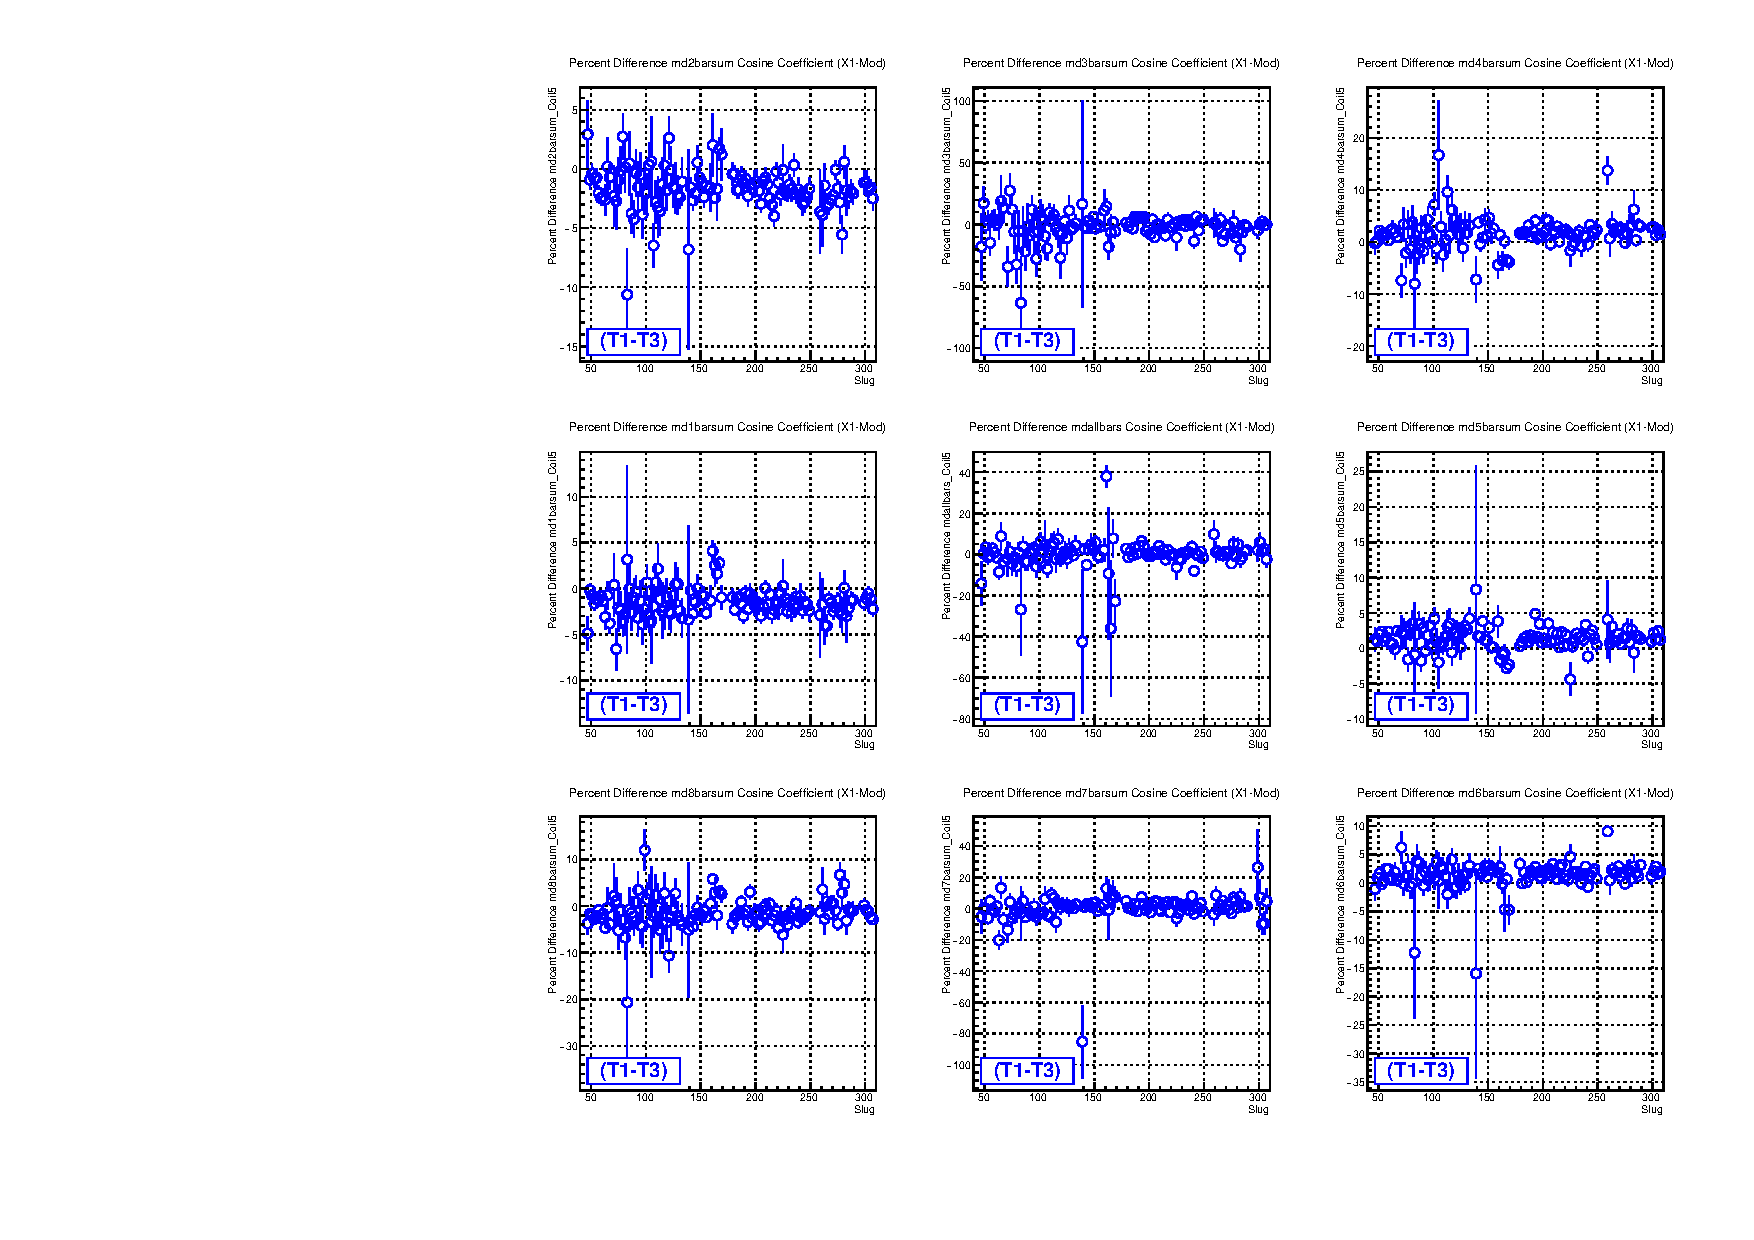
\includegraphics[width=5.6in]{Pictures/T1minusT3_mdallbars_coefficients_Coil5.pdf}}
\caption{Percent change in the out-of-phase (cosine) main detector response between data tertiles 1 and 3 during X1-modulation (coil 5). See Equation \ref{eq:fractional_tertile_change} for an explanation of the percent change shown.}
\label{fig:tert_md_coeff_coil5}
\end{figure}
\begin{figure}[h]

\centering
\framebox{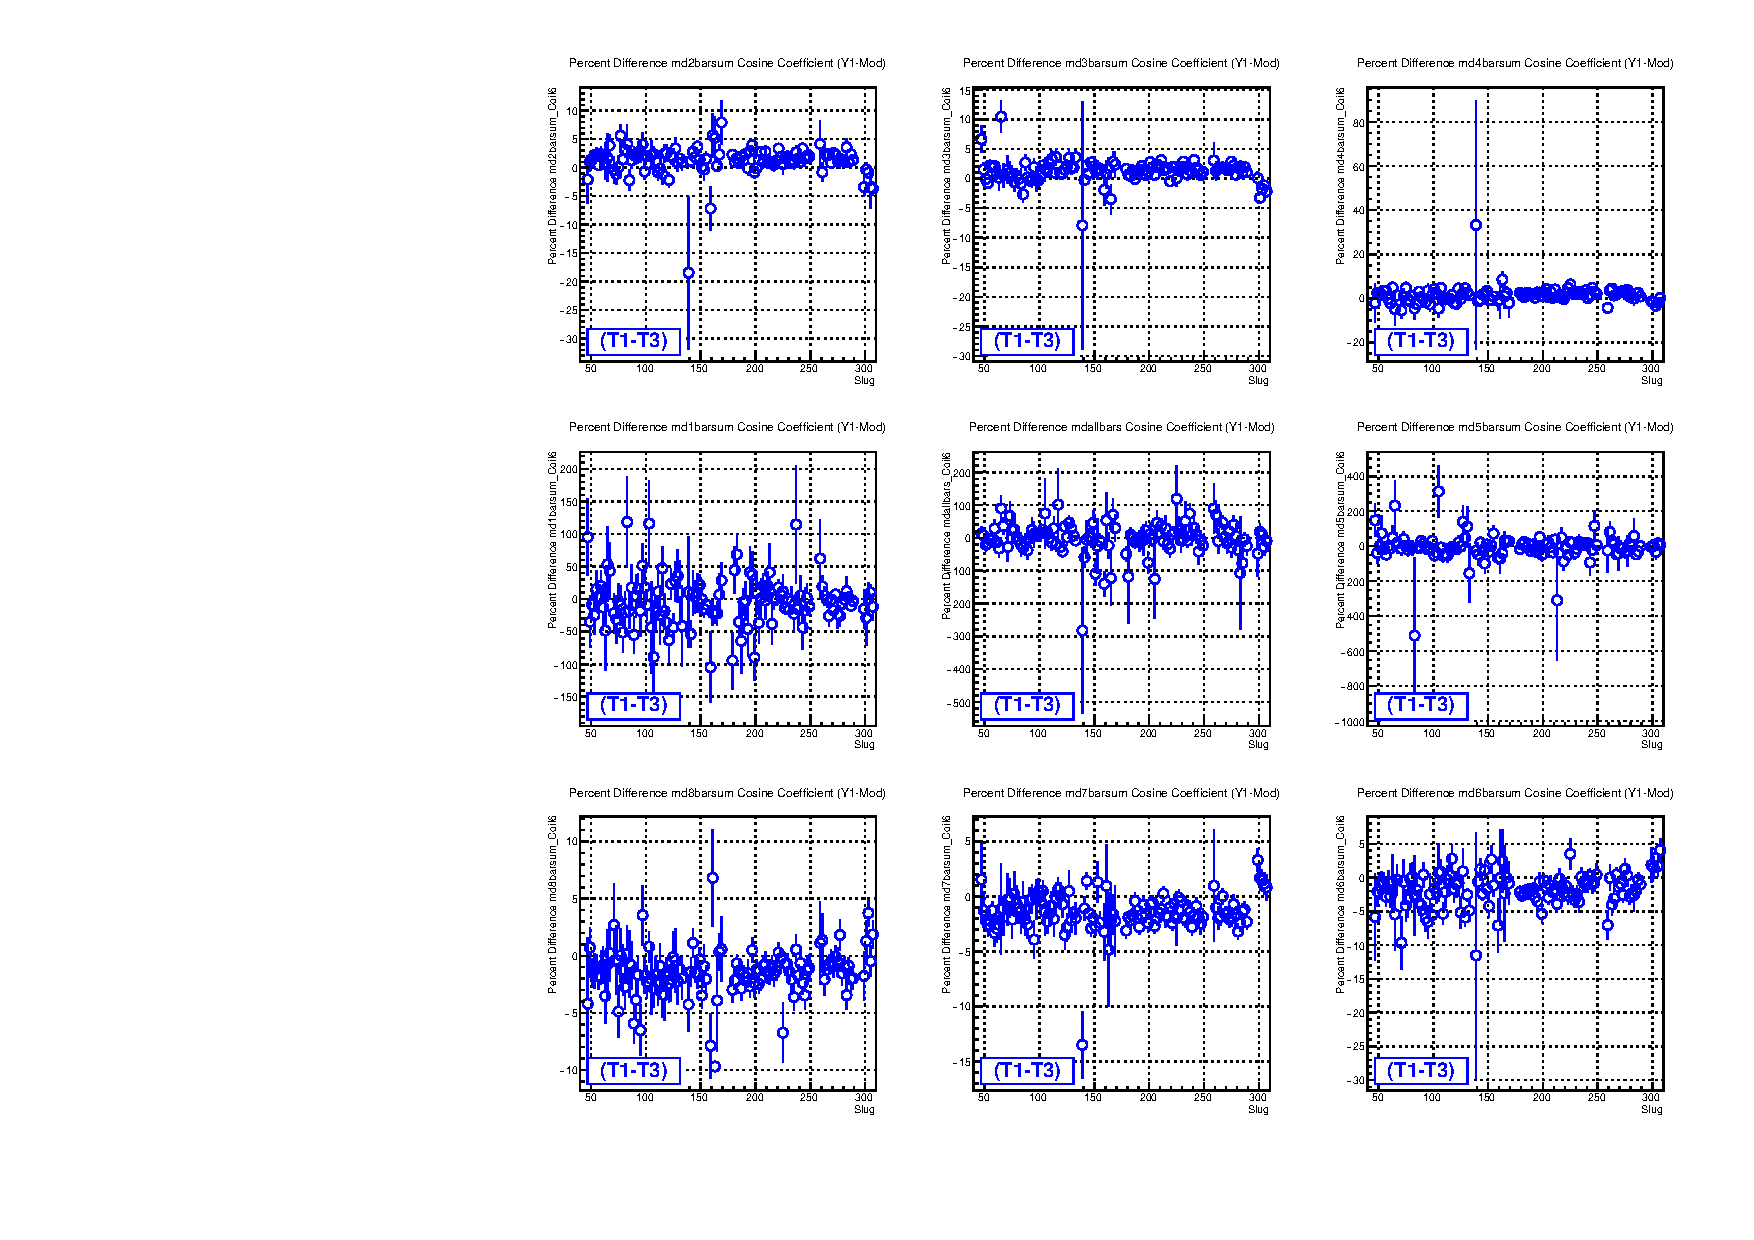
\includegraphics[width=5.6in]{Pictures/T1minusT3_mdallbars_coefficients_Coil6.pdf}}
\caption{Percent change in the out-of-phase (cosine) main detector response between data tertiles 1 and 3 during Y1-modulation (coil 6). See Equation \ref{eq:fractional_tertile_change} for an explanation of the percent change shown.}
\label{fig:tert_md_coeff_coil6}
\end{figure}
\begin{figure}[h]

\centering
\framebox{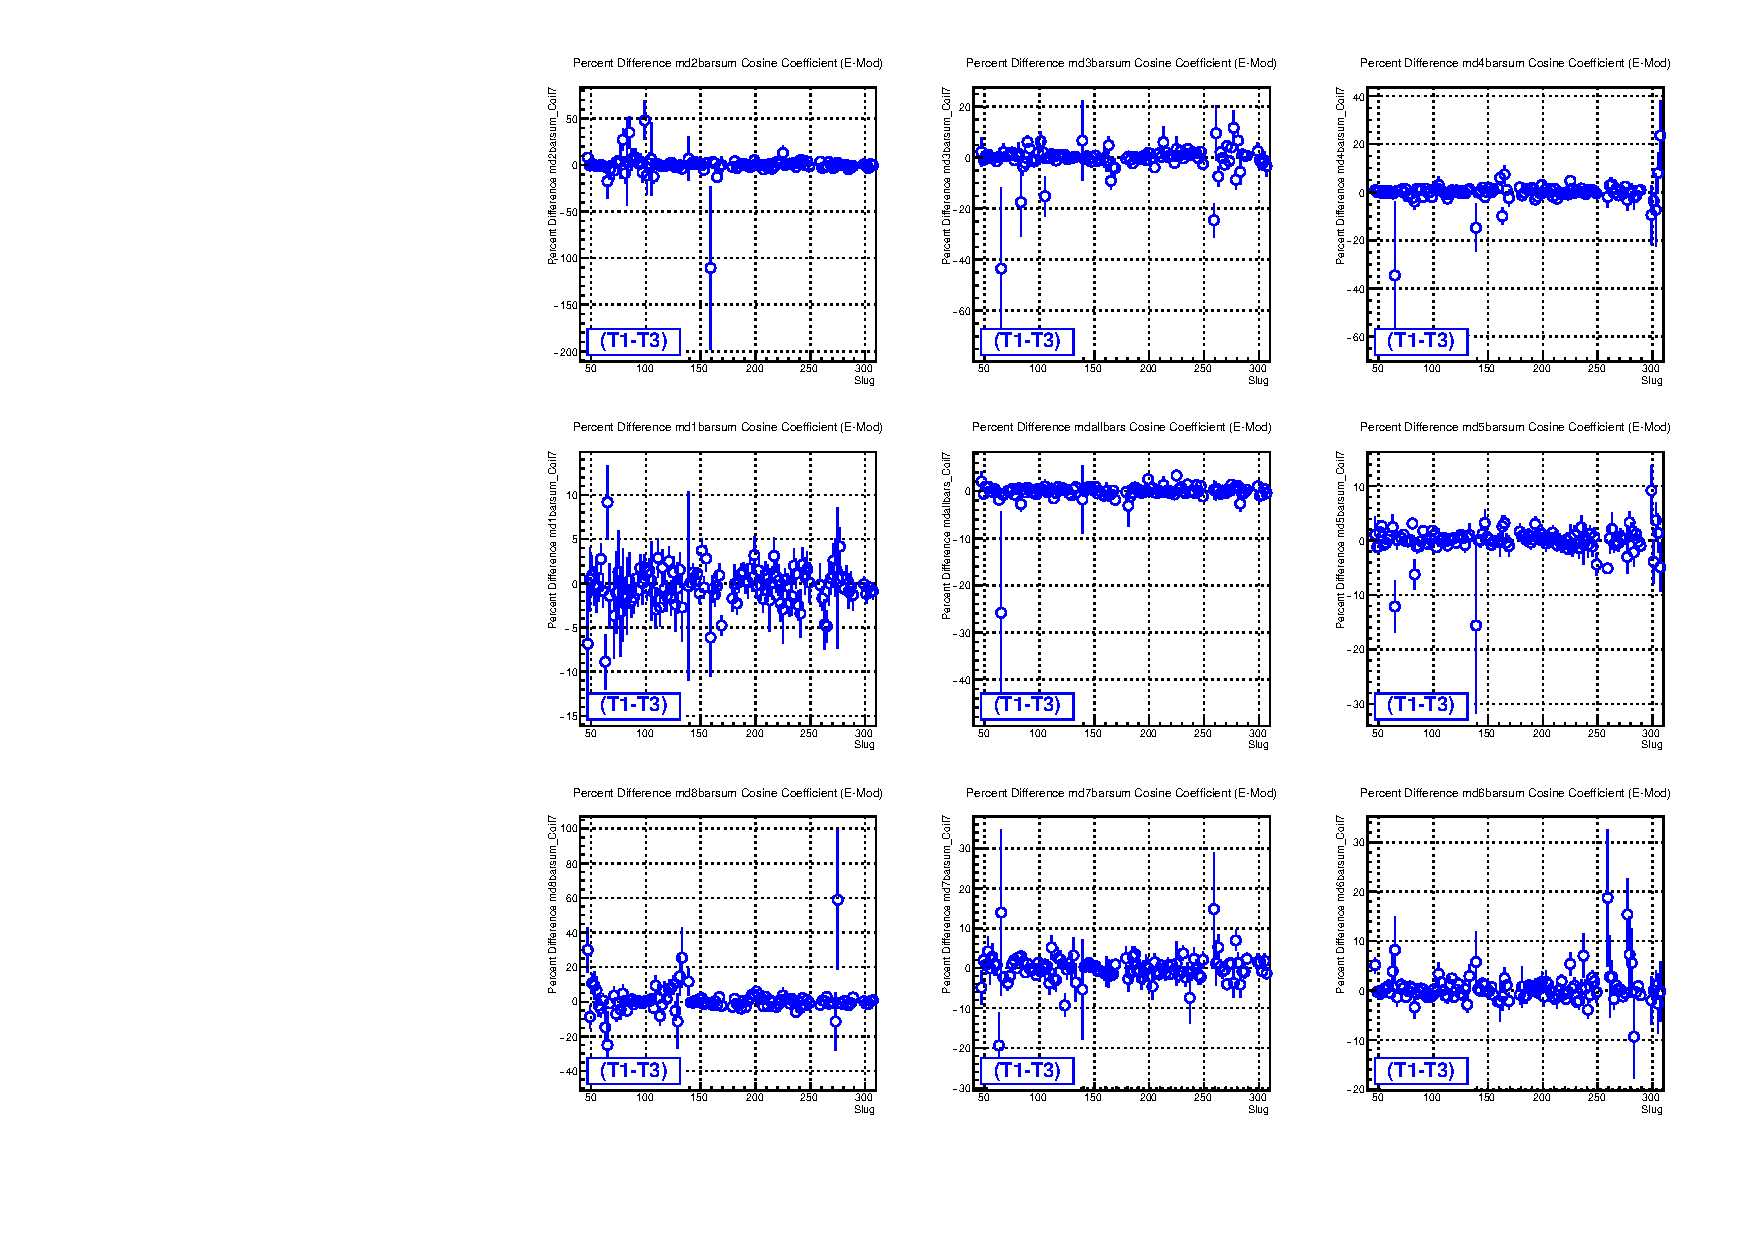
\includegraphics[width=5.6in]{Pictures/T1minusT3_mdallbars_coefficients_Coil7.pdf}}
\caption{Percent change in the out-of-phase (cosine) main detector response between data tertiles 1 and 3 during energy modulation(coil 7) . See Equation \ref{eq:fractional_tertile_change} for an explanation of the percent change shown.}
\label{fig:tert_md_coeff_coil7}
\end{figure}
\begin{figure}[h]

\centering
\framebox{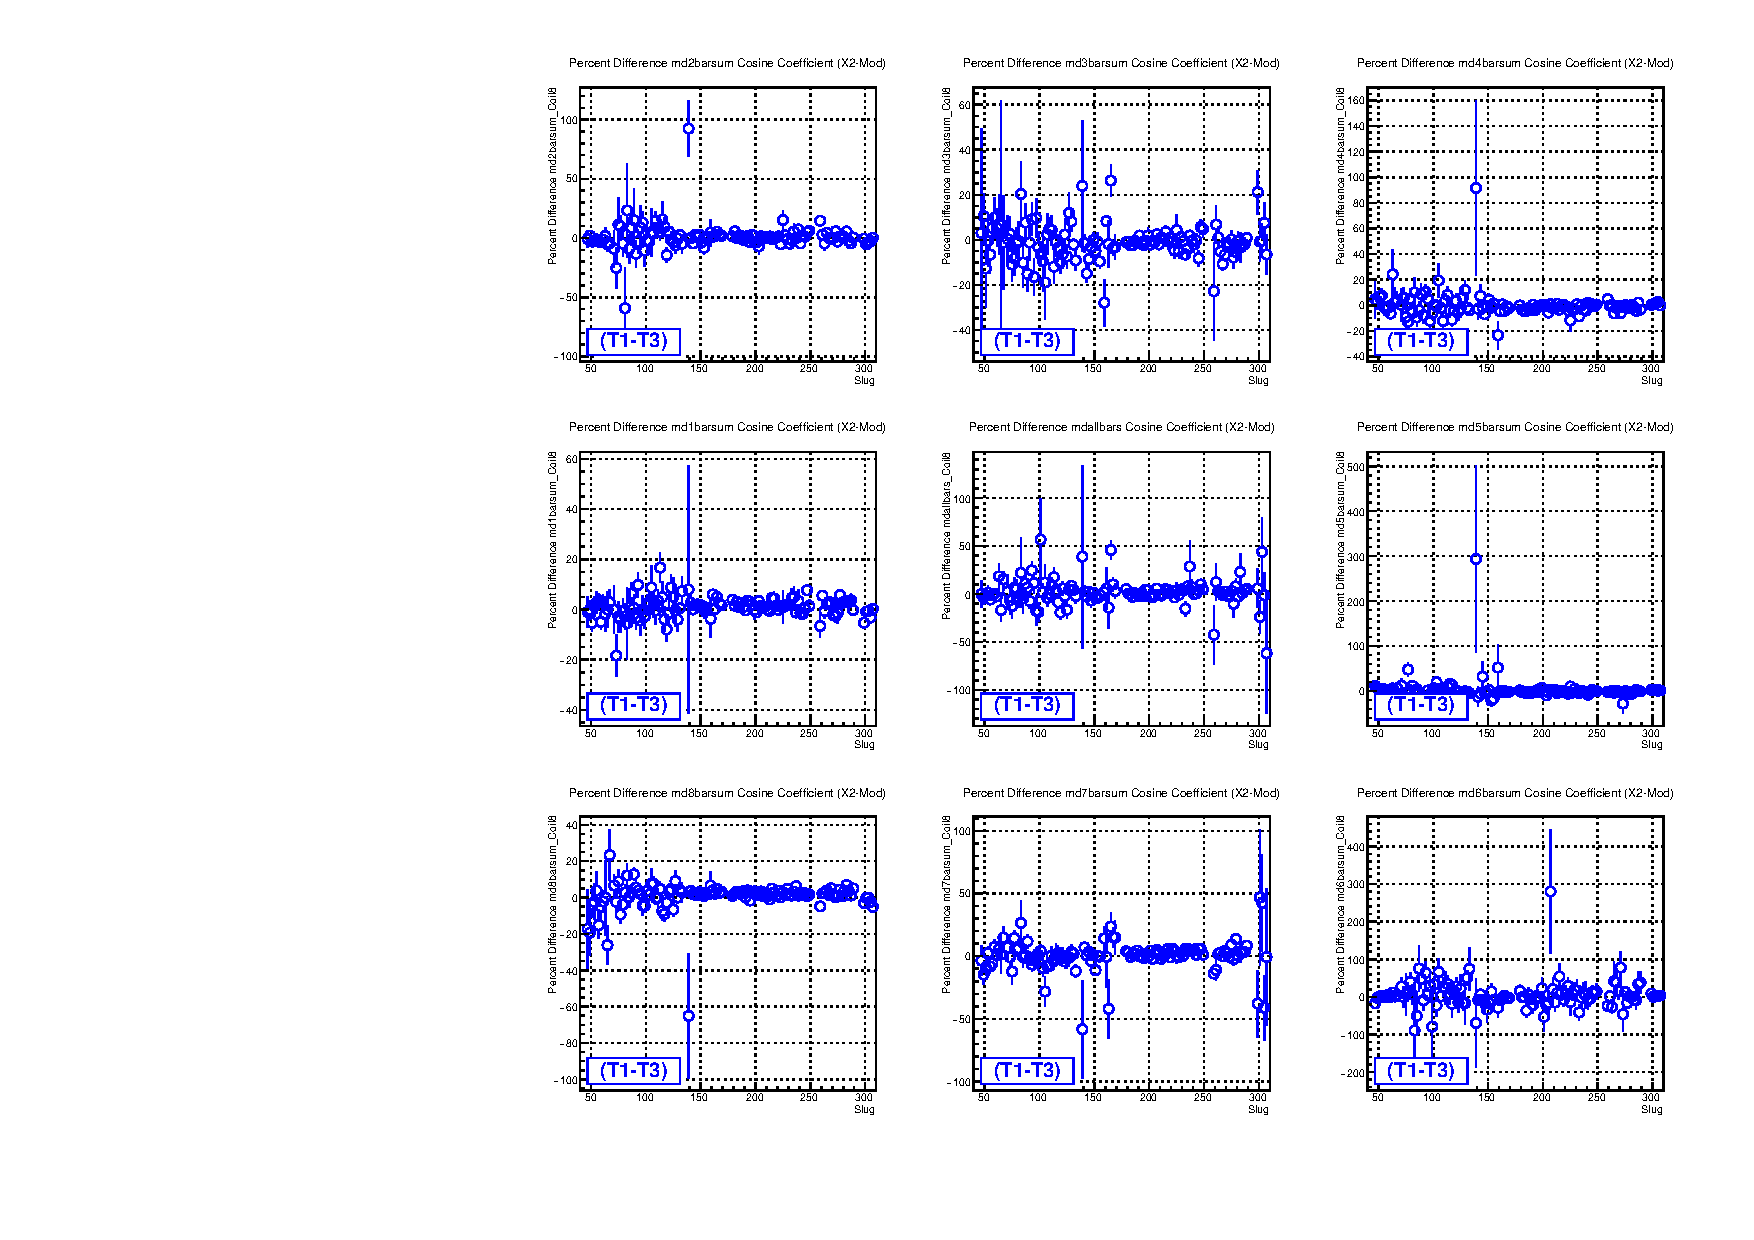
\includegraphics[width=5.6in]{Pictures/T1minusT3_mdallbars_coefficients_Coil8.pdf}}
\caption{Percent change in the out-of-phase (cosine) main detector response between data tertiles 1 and 3 during X2-modulation (coil 8). See Equation \ref{eq:fractional_tertile_change} for an explanation of the percent change shown.}
\label{fig:tert_md_coeff_coil8}
\end{figure}
\begin{figure}[h]

\centering
\framebox{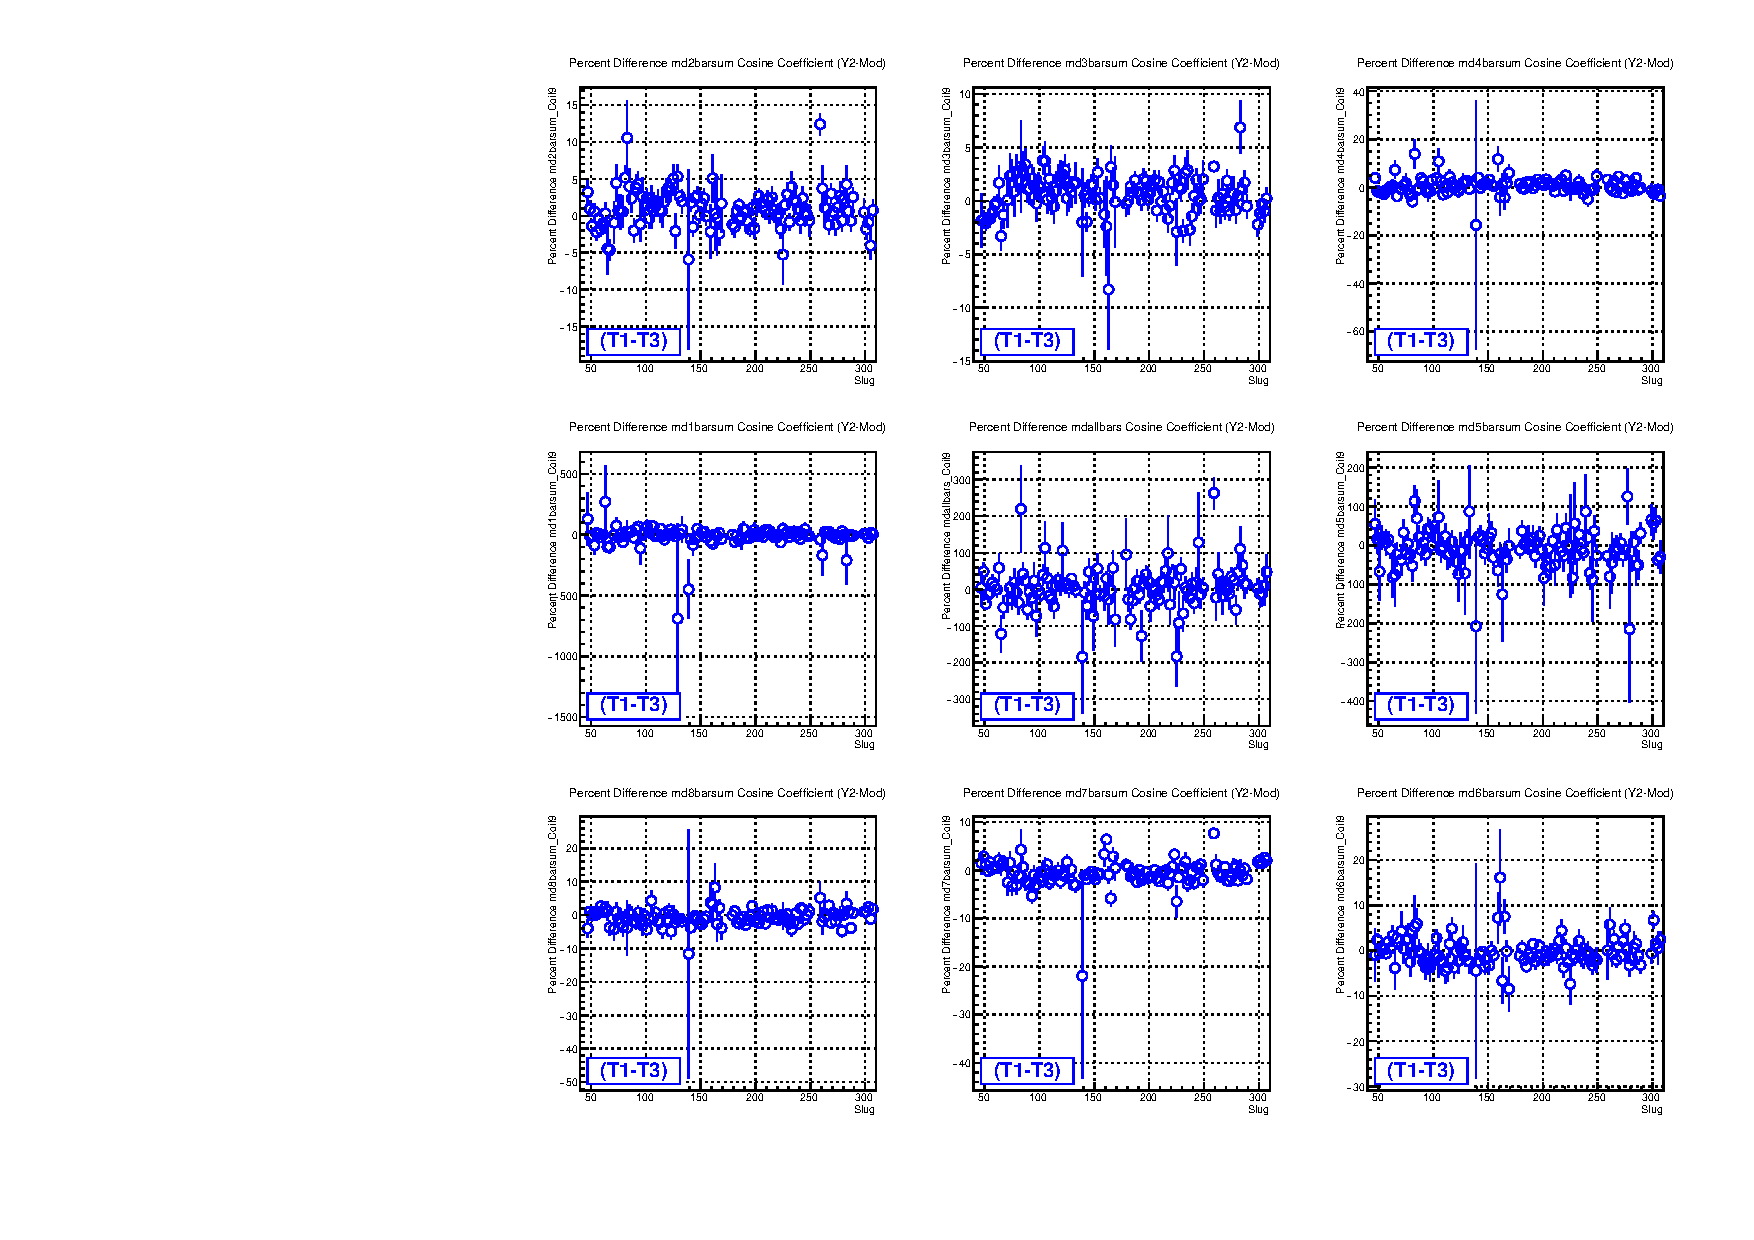
\includegraphics[width=5.6in]{Pictures/T1minusT3_mdallbars_coefficients_Coil9.pdf}}
\caption{Percent change in the out-of-phase (cosine) main detector response between data tertiles 1 and 3 during Y2-modulation (coil 9). See Equation \ref{eq:fractional_tertile_change} for an explanation of the percent change shown.}
\label{fig:tert_md_coeff_coil9}
\end{figure}
